

\documentclass{beamer}

\usetheme{Madrid}

\usepackage{graphicx,url}
\usepackage[utf8]{inputenc}
\usepackage[british,UKenglish,USenglish,english,american]{babel}
\usepackage[scaled]{helvet}
\usepackage[round]{natbib}
\usepackage[absolute,overlay]{textpos}
\usepackage{siunitx}
\sisetup{load-configurations = abbreviations}
\usepackage{multirow}
\usepackage{array}
\batchmode
\usepackage{amsmath,amssymb,enumerate,epsfig,bbm,calc,color,ifthen}
\usepackage{tikz, pdfpages}
\usetikzlibrary{calc,arrows,shapes,shapes.geometric,chains,backgrounds,fit,positioning, matrix}


\title[]{Control, diagnostics and estimation techniques for runaway electrons beams}

% A subtitle is optional and this may be deleted
\subtitle{XXX PhD Cycle}

\institute[Tor Vergata]{Università degli Studi di Roma "Tor Vergata"\\ 
\includegraphics[height=1cm,width=5cm]{senac-logo}}
\author[Mateusz Gospodarczyk]{Candidate: Mateusz Gospodarczyk\\ \\ Supervisor: Ph.D Daniele Carnevale\\ Co-supervisor: Dr. Basilio Esposito and Ph.D Luca Boncagni}





\AtBeginSubsection[]
{
  \begin{frame}<beamer>{Outline}
    \tableofcontents[currentsection,currentsubsection]
  \end{frame}
}

% Let's get started
\begin{document}

\begin{frame}
  \titlepage
\end{frame}

\begin{frame}{Outline}
  \tableofcontents
  % You might wish to add the option [pausesections]
\end{frame}


% -----------------------------------------------------------------------------
\section{Introduction}

\begin{frame}{Introduction}
\scriptsize
The study of the of the runaway electron (REs) and RE beams mitigation techniques is the goal of this Ph.D work.
\begin{block}{REs and RE beam}
	\begin{itemize}
	\item Are beams of electrons within a tokamak plasma, accelerated to relativistic velocities.
	\item RE beams might be formed during disruptions and could carry a large fraction of ohmic current leading to deep melting of the vessel in case of impact.
	\item They represent a major concern in tokamaks (ITER) since RE beam current up to 13MA could be formed after disruptions leading to potentially unrecoverable damages
	\end{itemize} 
\end{block}

\begin{columns}
    \begin{column}{0.7\textwidth}
        \centering
        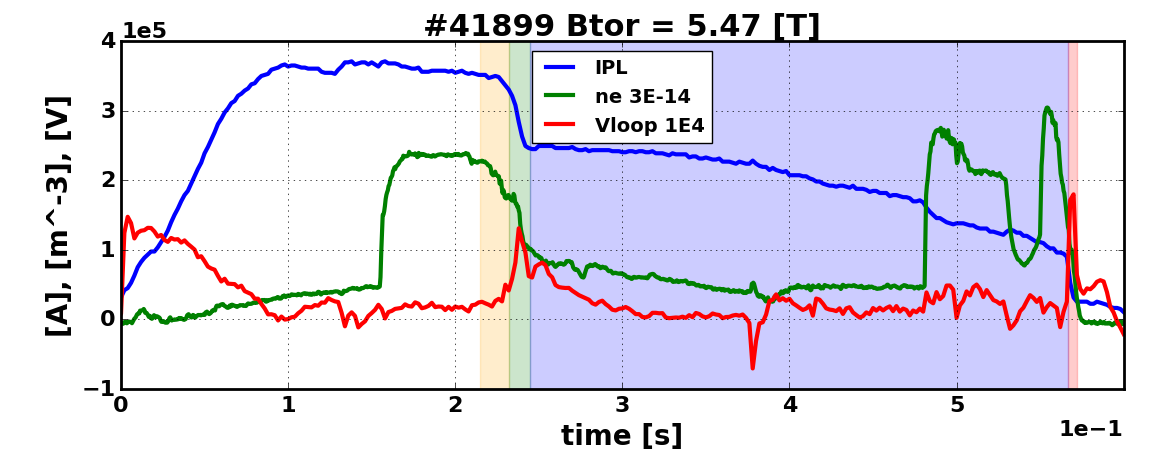
\includegraphics[width=1\linewidth]{fig/41899_ipl} 
    \end{column}
    
    \begin{column}{0.3\textwidth}  %%<--- here
        \only <1>{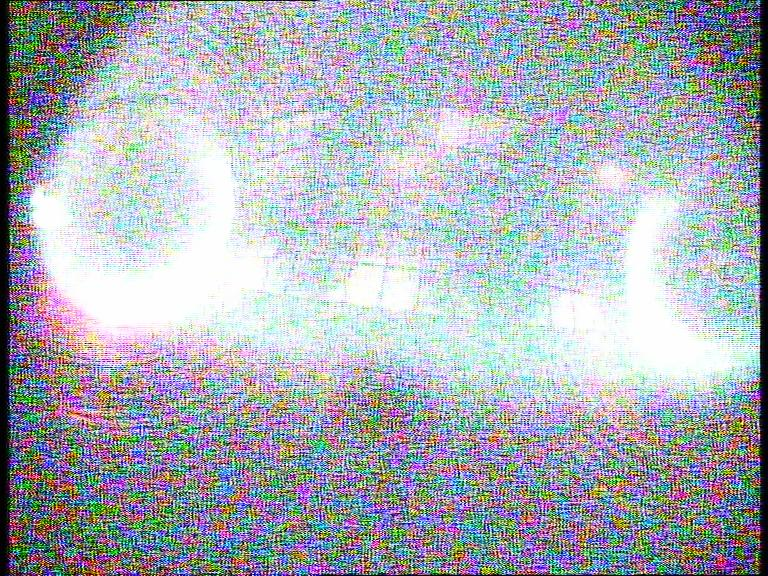
\includegraphics[width=1\linewidth]{frame/3}\\$110$ ms}
        \only <2>{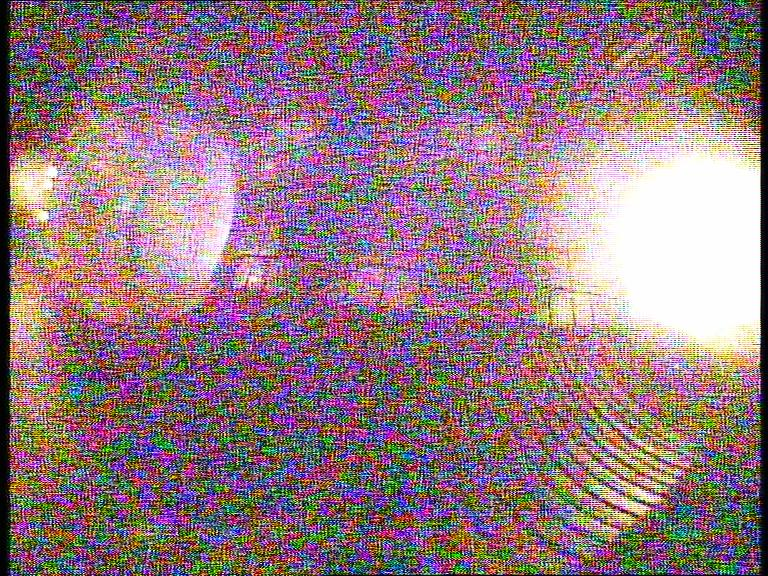
\includegraphics[width=1\linewidth]{frame/10}\\$390$ ms}
        \only <3>{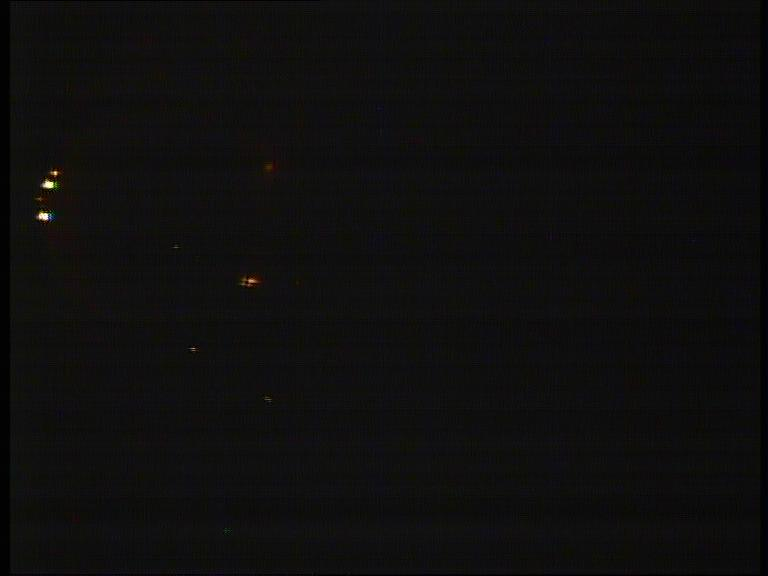
\includegraphics[width=1\linewidth]{frame/15}\\$590$ ms}
    \end{column}
\end{columns} 

\end{frame}

\begin{frame}{Introduction}
    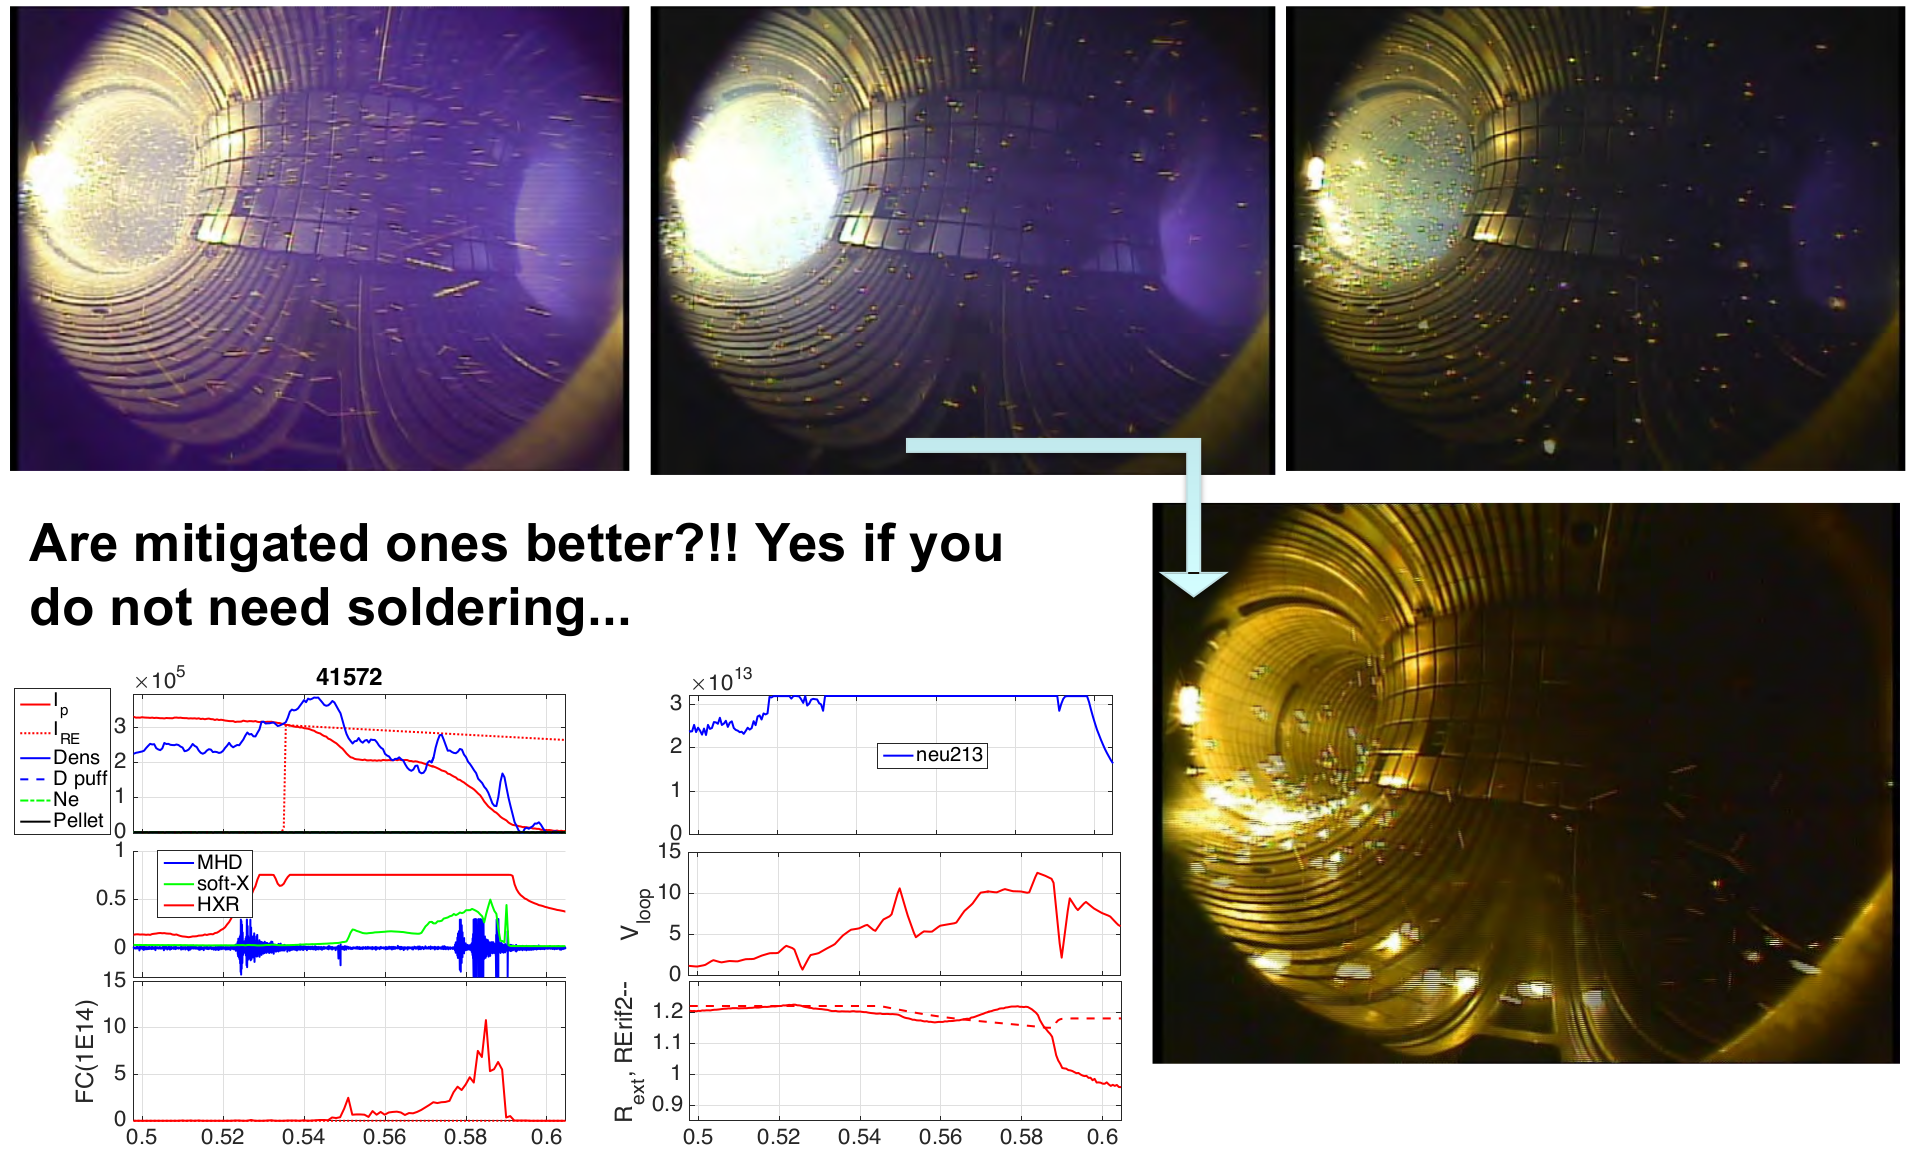
\includegraphics[width=1\linewidth]{frame/melting.png}
\end{frame}



\begin{frame}{Introduction}
\scriptsize
REs mitigation is one task of the Medium Size Tokamak (MST-1) RE experiments in support of ITER (International Thermonuclear Experimental Reactor and Latin for "the way").
\centering
\begin{block}{Research goal}

\begin{itemize}
	\item REs Diagnostics: Real-time interferometer (RE beam position) and   REIS system (synchrotron radiation).
	\item Runaway Electron Control System (RECS) framework.
\end{itemize} 
\end{block}



This work is based on the collaboration with different research groups from tokamak experiments.
\begin{figure}
\centering
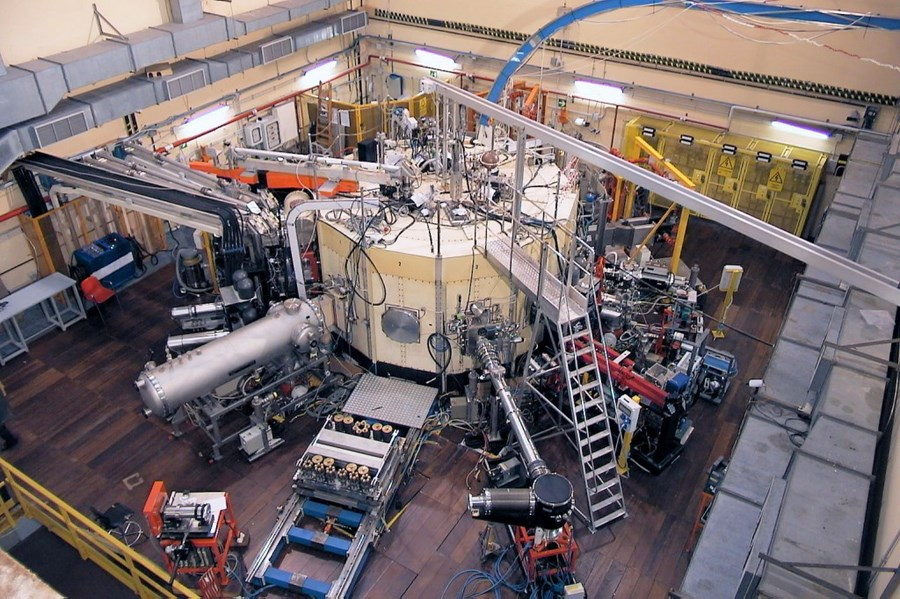
\includegraphics[width=0.2\linewidth]{tokamak/ftu} 
\hspace{0.1cm}
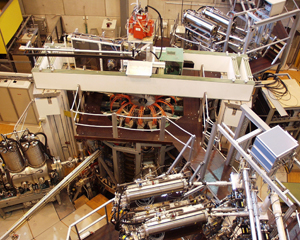
\includegraphics[width=0.2\linewidth]{tokamak/TCV_1}
\hspace{0.1cm}
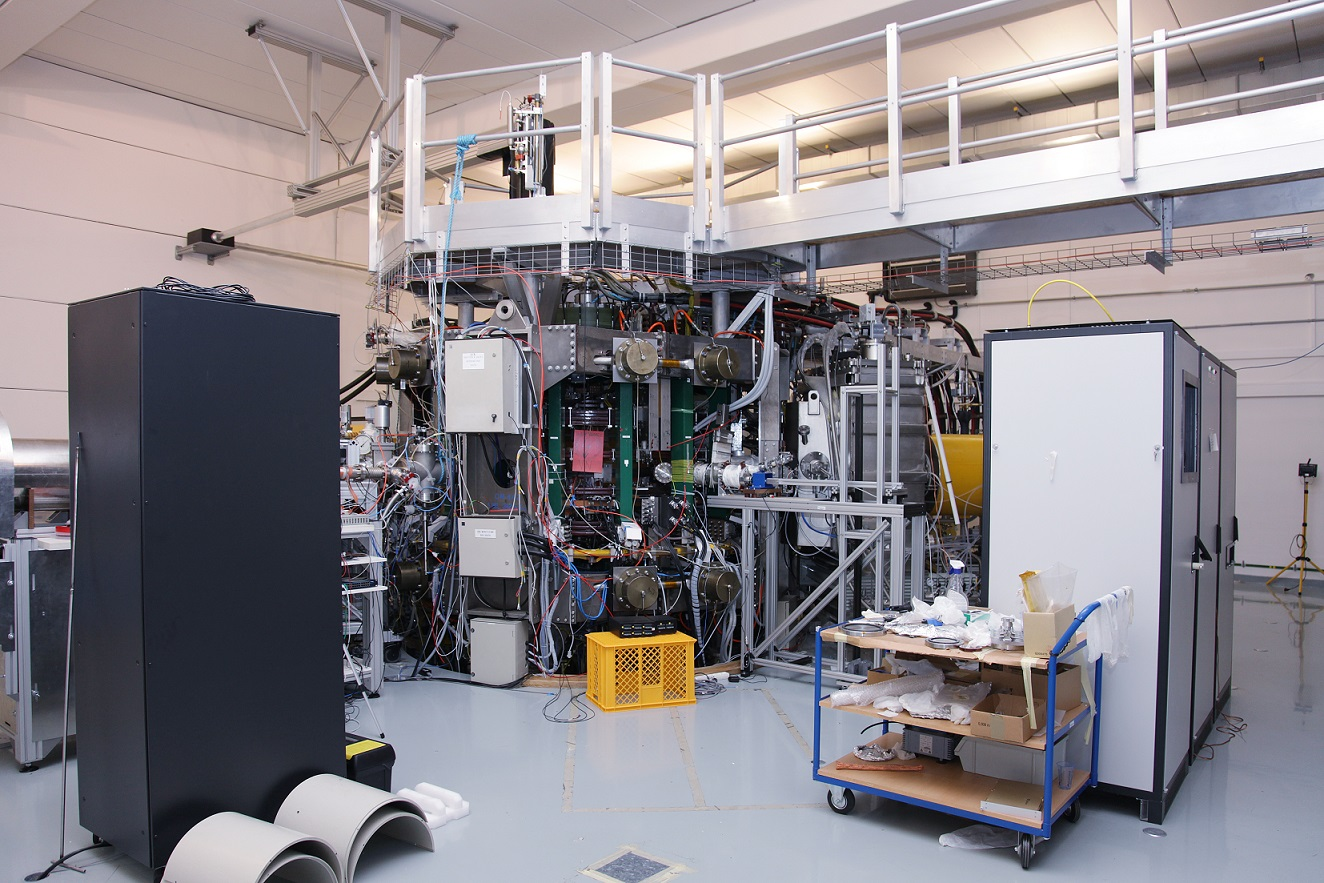
\includegraphics[width=0.2\linewidth]{tokamak/COMPASS}
\hspace{0.1cm}
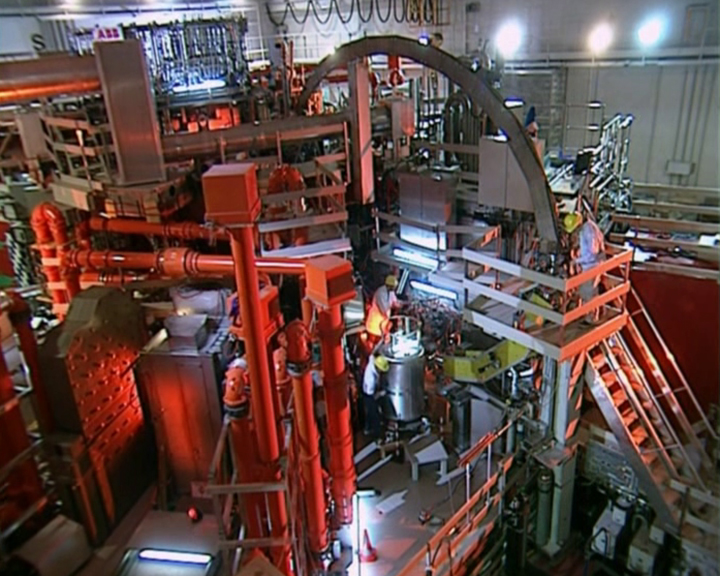
\includegraphics[width=0.2\linewidth]{tokamak/asdex}
\end{figure}

\begin{textblock*}{10pt}(40pt,220pt)
\textbf{FTU}
\end{textblock*}
\begin{textblock*}{10pt}(120pt,220pt)
\textbf{TCV}
\end{textblock*}
\begin{textblock*}{10pt}(190pt,220pt)
\textbf{COMPASS}
\end{textblock*}
\begin{textblock*}{10pt}(270pt,220pt)
\textbf{ASDEX}
\end{textblock*}



\end{frame}


%-----------------------------------------------------------------------------
\section{REs and RE beam}

\begin{frame}[allowframebreaks]{REs Generation}
\scriptsize
The decrease of the Coulomb collisions frequency lead to an unbalance in the equilibrium between collisional force $F_C$ and gain force $F_G$ that accelerated the electrons up to relativistic speed.
\begin{itemize}
	\item  A simple treatment of the RE generation problem \cite{paz2014growth}, 0-D modeling,
	\begin{equation}
	\dot{n}_{RE} = S_{pri} + \gamma_{sec}(n_{RE})
	\end{equation}
    where $S_{pri} = f(T_{e},n_e,E_{||},Z_{eff})$ is the primary REs generation (Dreicer) while $\gamma_{\text{A}}(n_{RE})$ is the secondary generation and $\gamma_{\text{A}}$ is the avalanche multiplication factor.\\
    If the electric field is above the Dreicer field $E_D$ then the electrons starts to accelerate up to the speed of light.
    \begin{equation}
    \label{eq:DreicerForce}
     E_D = \frac{n_e e^3 ln \Lambda}{4 \pi \epsilon^2_0 T_e}
    \end{equation} 
    where $T_e$ is the electron temperature \si{\eV}.\\
    The generation of REs in avalanche mechanism through knock-on collisions.
    The avalanche growth rate can be expressed, as done in \cite{PutvinskiRosenbluth} as:
    \begin{equation}
     \label{eq:PutvinskiRosenbluth}
     \dot{n}_{RE} \approx \frac{n_{RE}(E-1)}{\tau \ln (\Lambda)} \sqrt{\frac{\pi \Phi}{3(Z_{eff} + 5)}} \left(1-E^{-1}+\frac{4\pi(Z_{eff}+1)^2}{3\Phi(Z_{eff}+5)(E^2+4/\Phi^2-1)}\right)^{0.5}
    \end{equation}
    where $\Phi = (1+1.46\epsilon^0.5+1.72\epsilon)^{-1}$ and $\epsilon = \frac{r}{R}$ is the inverse aspect ratio.\\

	\item REs are possible if the  parallel electric field is greater than
	Critical electric field $E_C$ (\cite{connor1975relativistic}):
	\begin{equation}
	\label{eq:criticalElectricField}
	E_c = \frac{F_{ee}}{e} = \frac{n_e e^3 ln \Lambda}{4 \pi \epsilon^2_0 m_e c^2}
	\end{equation}
	\item RE suppression experiments performed on FTU suggest that the suppression of REs occurs at electric fields higher that the above mentioned \cite{Esposito2016}.
	\begin{equation}
	\frac{E_C^{synch}}{E_C} \approx 1+C(Z_{eff}) F_{gy}^{\alpha}
	\end{equation}
	where $\alpha = 0.45 \pm 0.03$, $F_{gy} = \frac{2 \epsilon_0 B_0^2}{3 n_e ln \Delta m_e} $ and $C(Z_{eff}) \approx 1.64 + 0.53 Z_{eff} - 0.015 Z_{eff}^2 $.
\end{itemize}

\end{frame}


\begin{frame}{REs: electron energy}
\scriptsize

The prediction electron energy $W$ can be found \cite{Martin-Solis2010} by integrating
\begin{align*}
P_{tot} &= \frac{d W}{dt} = P_{gain} - P_{coll} - \color{blue}{P_{synch}} \color{black}{}= e \frac{V_{loop}}{2 \pi R} v_{||} - \frac{n_e e^4 ln \Lambda}{4 \pi \epsilon^2_0 m_e v}- \color{blue}{\underbrace{\frac{2}{3} r_e m_e c^3 \beta^4 \gamma ^4 \frac{1}{\left< R^2_{g}(t)\right>}}_\text{REIS}} \nonumber   \nonumber 
\end{align*}

    \begin{figure}
	    \vspace*{-0.6cm}
	    %\hspace*{2.5cm}
	    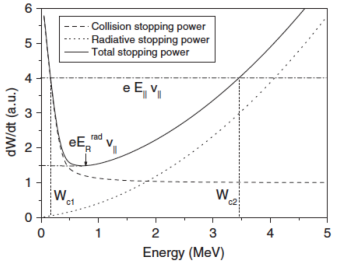
\includegraphics[width=0.6\linewidth]{drive/total_power_emitted.png}
	\end{figure}
	
\end{frame}
\begin{frame}{REs: energy evolution}
	
	\scriptsize
	\begin{columns}
        \begin{column}{0.4\textwidth}
               \begin{itemize}
                \item In Dreicer region (green line), the electrons with energies $W$ between $W_{C1}$ and $W_{C2}$ will be accelerated up to $W_{C2}$.
                \item If $E_{||}$ is below the Dreicer field (red line) then electron will be decelerated to $W_{c1*}$ (\textbf{{\color{red}suppression}}). 
                \item If the electric field is above the Dreicer field (blue line) then the thermal electron will be accelerated to $W_{c2*}$ (\textbf{{\color{blue}generation}})
            \end{itemize}
        \end{column}
        
        \begin{column}{0.6\textwidth}  %%<--- here
        
        \begin{figure}
            \vspace*{-0.6cm}
            \centering
        	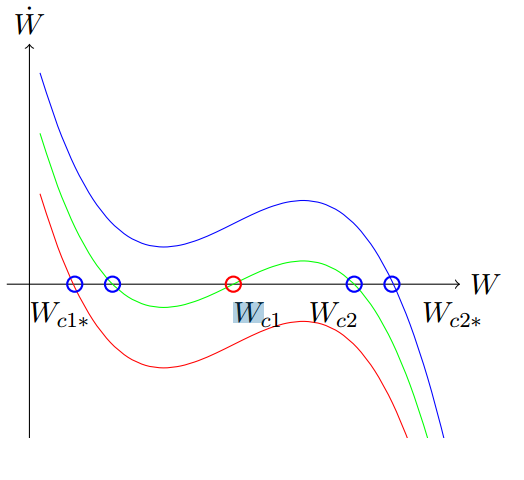
\includegraphics[width=1\linewidth]{Chapter2Fig/energy_evolution.png}

        \end{figure}

        \begin{textblock*}{10pt}(270pt,130pt)
         $\upuparrows$\textbf{U}
        \end{textblock*}

        \begin{textblock*}{10pt}(210pt,175pt)
         $\downdownarrows$\textbf{U}
        \end{textblock*}
        
        \end{column}
    \end{columns}  

\end{frame}

\begin{frame}{REs: hysteresis phenomena}
    \scriptsize
    In order to characterize the hysteresis phenomena a specific matlab routine has been implemented for the analysis of FTU database (650 pulses)
    \begin{figure}
        \vspace*{-0.4cm}
        \centering
    	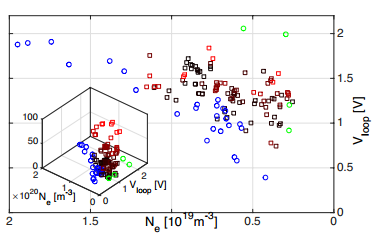
\includegraphics[width=0.6\linewidth]{Chapter2Fig/hysteresis2.png}
        \vspace*{-0.6cm}
    \end{figure}
    REs generation (green circles) and suppression (blue circles). REs discharges with different number/energy of REs are represented by squares colored from black (no REs) to red (high RE energy). The squares represent values of shots in stationary plasma conditions in which the density, $I_P$, $V_{loop}$ and NEU213 signals have a small standard deviations within a time window of 120 \si{\ms}.

\end{frame}



\begin{frame}{REs diagnostics}
    \scriptsize
    Plasma diagnostics are crucial in fusion devices since their measurements are required for \textbf{machine protection}, \textbf{plasma control} and \textbf{physics studies}.
    \begin{block}{Plasma diagnostics on FTU}
     \scriptsize	
     Integration of different diagnostics for REs measurements and new software tools within the FTU real-time plasma control system is contributing to the characterization of the RE dynamics and to the study of possible mitigation strategies.
    	\scriptsize
    	\begin{itemize}
    		\item Development and improvement of \textbf{REIS} (RE  Imaging  and  spectroscopy system) system  to detect and study the in-flight REs energy spectrum.
    		\item Real-time elaboration system for \textbf{two-color medium-infrared scanning interferometer} for electron density measurements
    	\end{itemize}
    \end{block}
\end{frame}





%------------------------------------------------------------------------------
\section{REIS SYSTEM}
\begin{frame}[allowframebreaks]{REIS SYSTEM: Introduction}

\begin{figure}
\centering
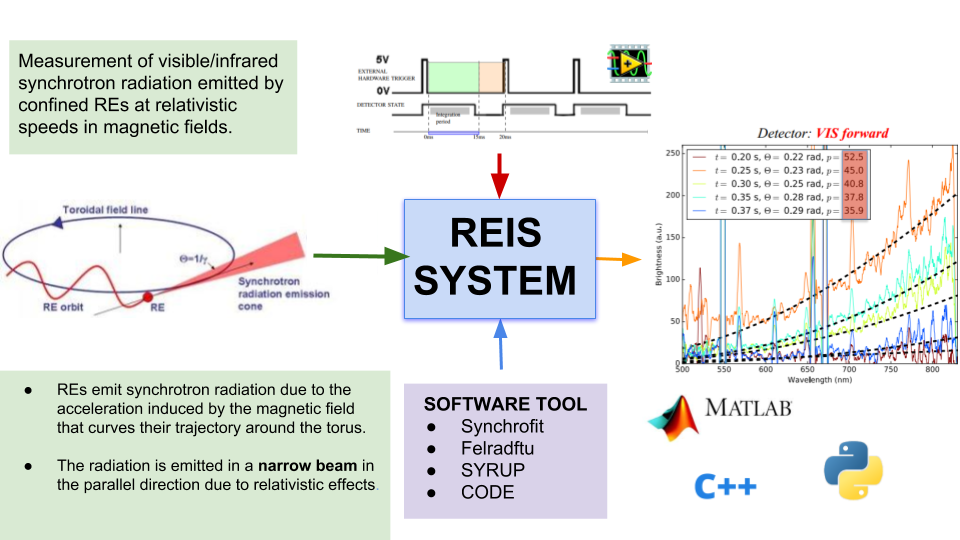
\includegraphics[width=1\textwidth]{drive/REISintro.png}
\end{figure} 


\end{frame}





\begin{frame}{REIS SYSTEM: Experimental set-up}
\scriptsize
\small
\begin{figure}
	\centering
    \vspace*{-0.5cm}
	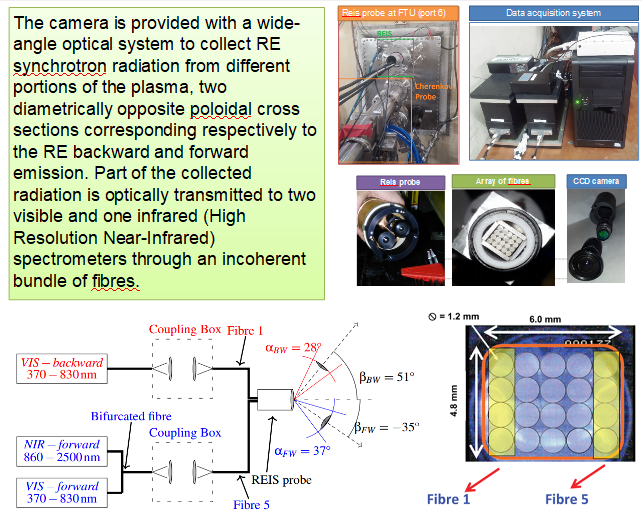
\includegraphics[width=0.8\textwidth]{drive/setup.png}
\end{figure}
\end{frame}

\begin{frame}{REIS SYSTEM: Technical Details}
\scriptsize
\begin{figure}
	\centering
	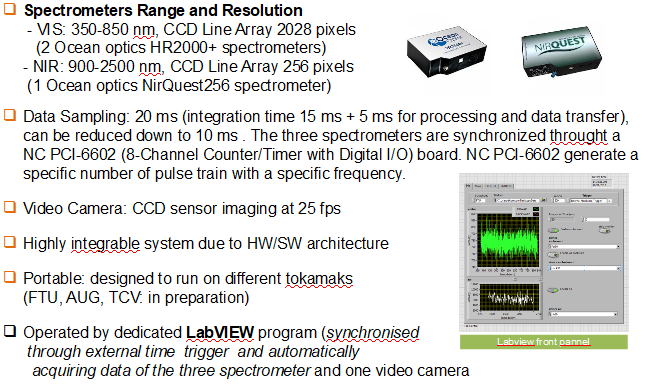
\includegraphics[width=0.9\textwidth]{drive/tecnicalreis.png}
\end{figure}
\end{frame}

\begin{frame}{REIS SYSTEM: Calibration}
\begin{figure}
	\centering
	\only<1>{
	    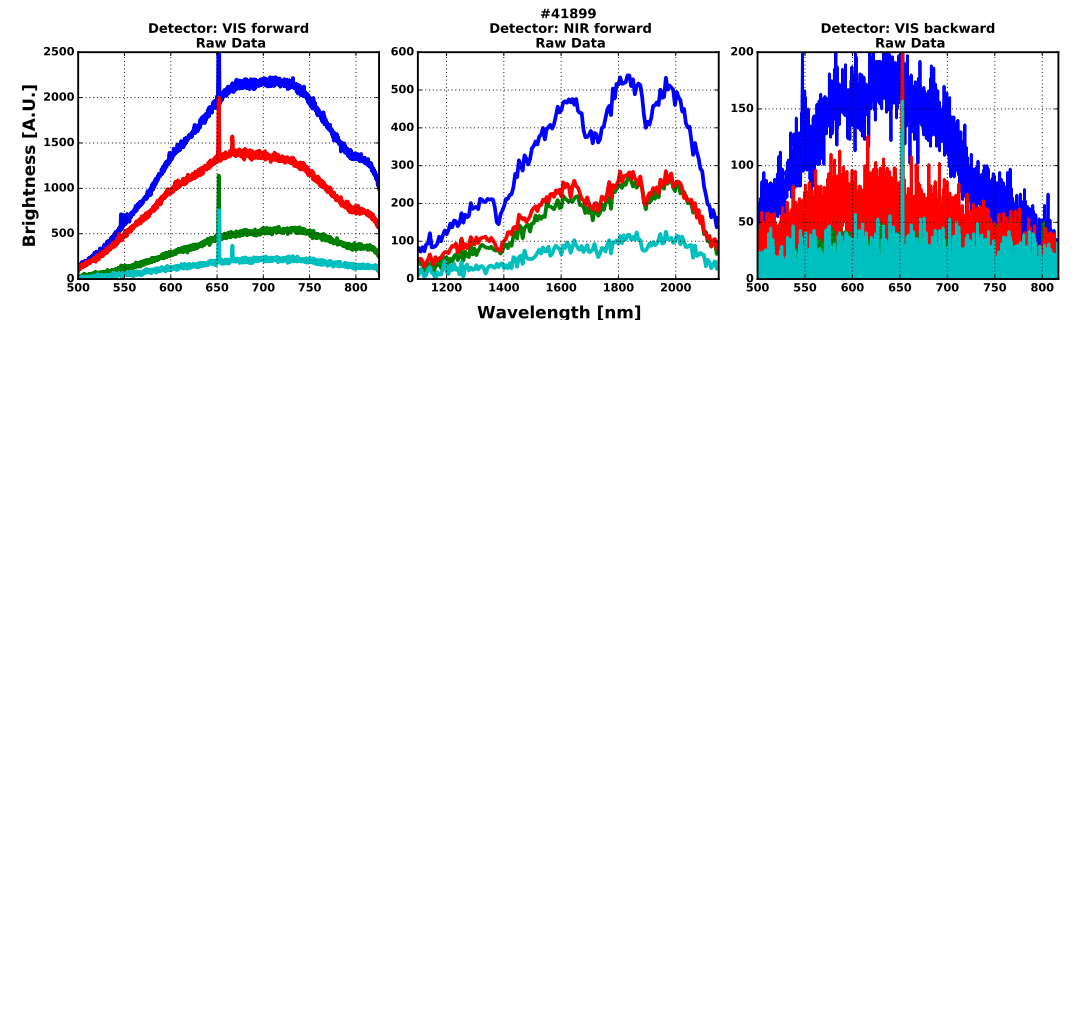
\includegraphics[width=0.7\textwidth]{chapterreisfig/calibTotal1.png}
	}
	\only<2>{
	    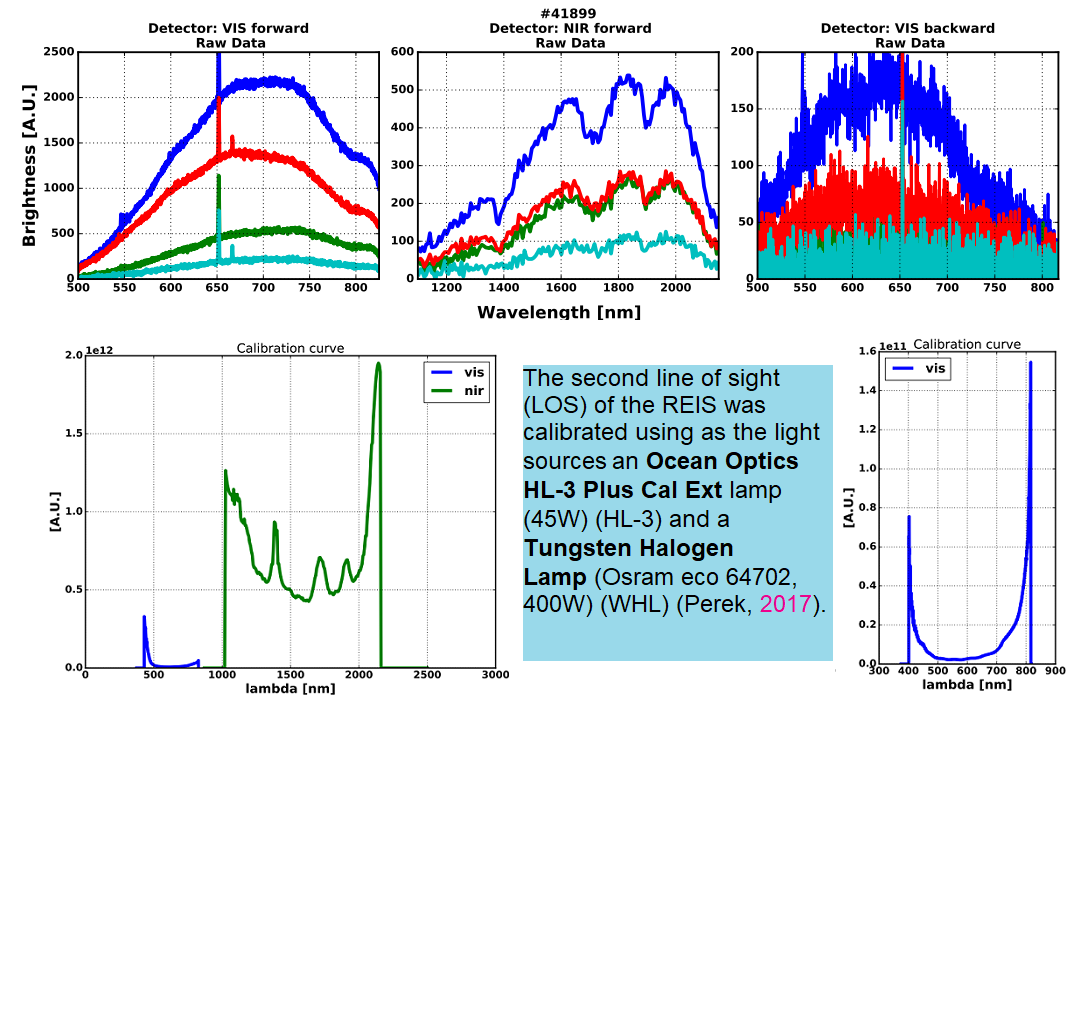
\includegraphics[width=0.7\textwidth]{chapterreisfig/calibTotal2.png}
	}
	\only<3>{
	    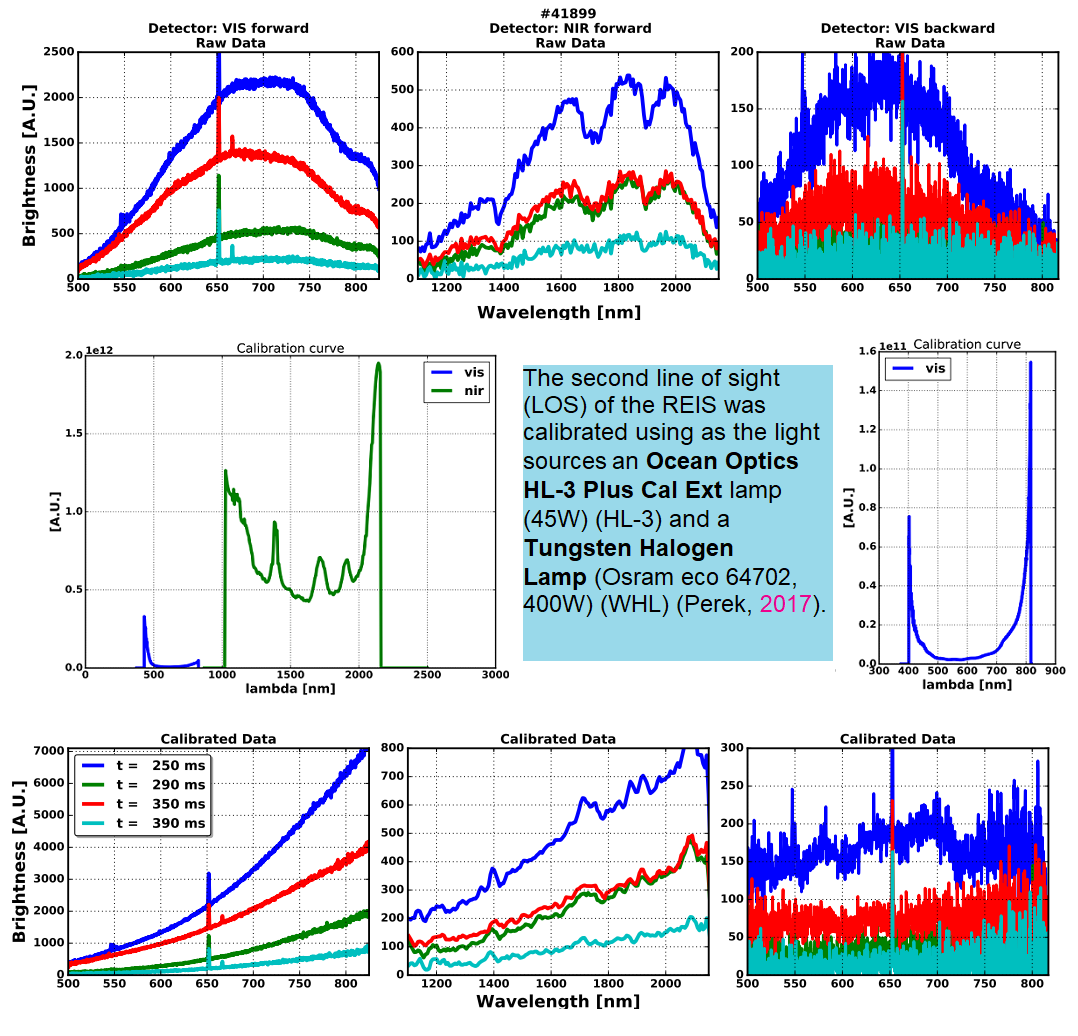
\includegraphics[width=0.7\textwidth]{chapterreisfig/calibTotal.png}
	}
\end{figure}
\end{frame}


\begin{frame}[t]{Energy Estimation: Synchrofitroutine}
    \scriptsize
    Energy estimation: the routine create a model by lmfit python routine which provide a complex fitting models for non-linear least-squares problem that wraps the brightness
    \begin{figure}
    
    	\begin{center}
    		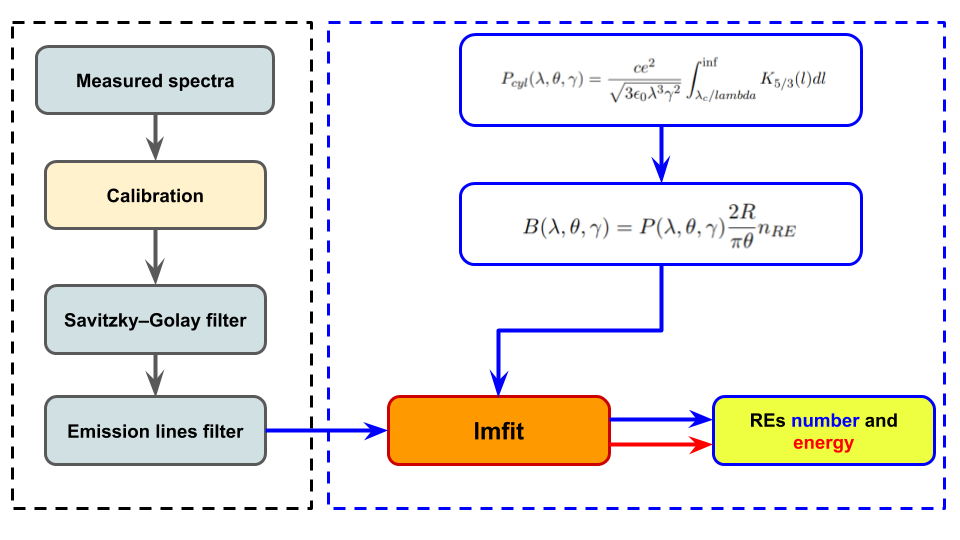
\includegraphics[width=0.8\textwidth]{drive/sychrofitRoutine.png}
    	\end{center}
    \end{figure}
    
\end{frame}


\begin{frame}{FTU: Experimental results}

    \only<1>{
    
        \begin{columns}
        
        \begin{column}{0.5\textwidth}
        \begin{figure}
            \vspace*{-1cm}
        	\begin{center}
        		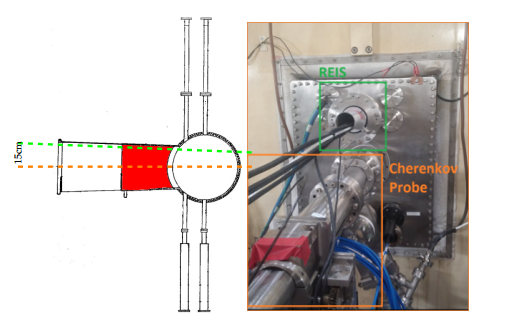
\includegraphics[width=1\textwidth]{chapterreisfig/ftu_port.png}\\
        	    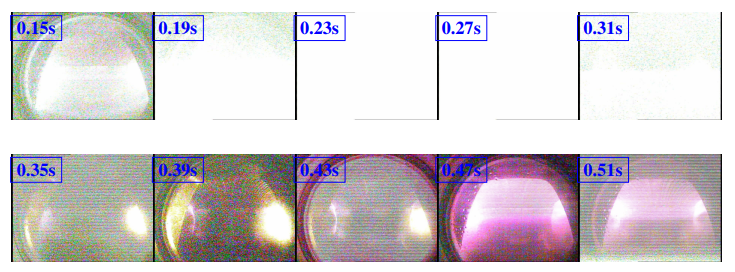
\includegraphics[width=1\textwidth]{chapterreisfig/ftu/image41899_.png}
        	\end{center}
        \end{figure}
        
        
        \end{column}
        
        \begin{column}{0.5\textwidth}  %%<--- here
        
        \begin{figure}
            \vspace*{-1cm}
        	\begin{center}
                  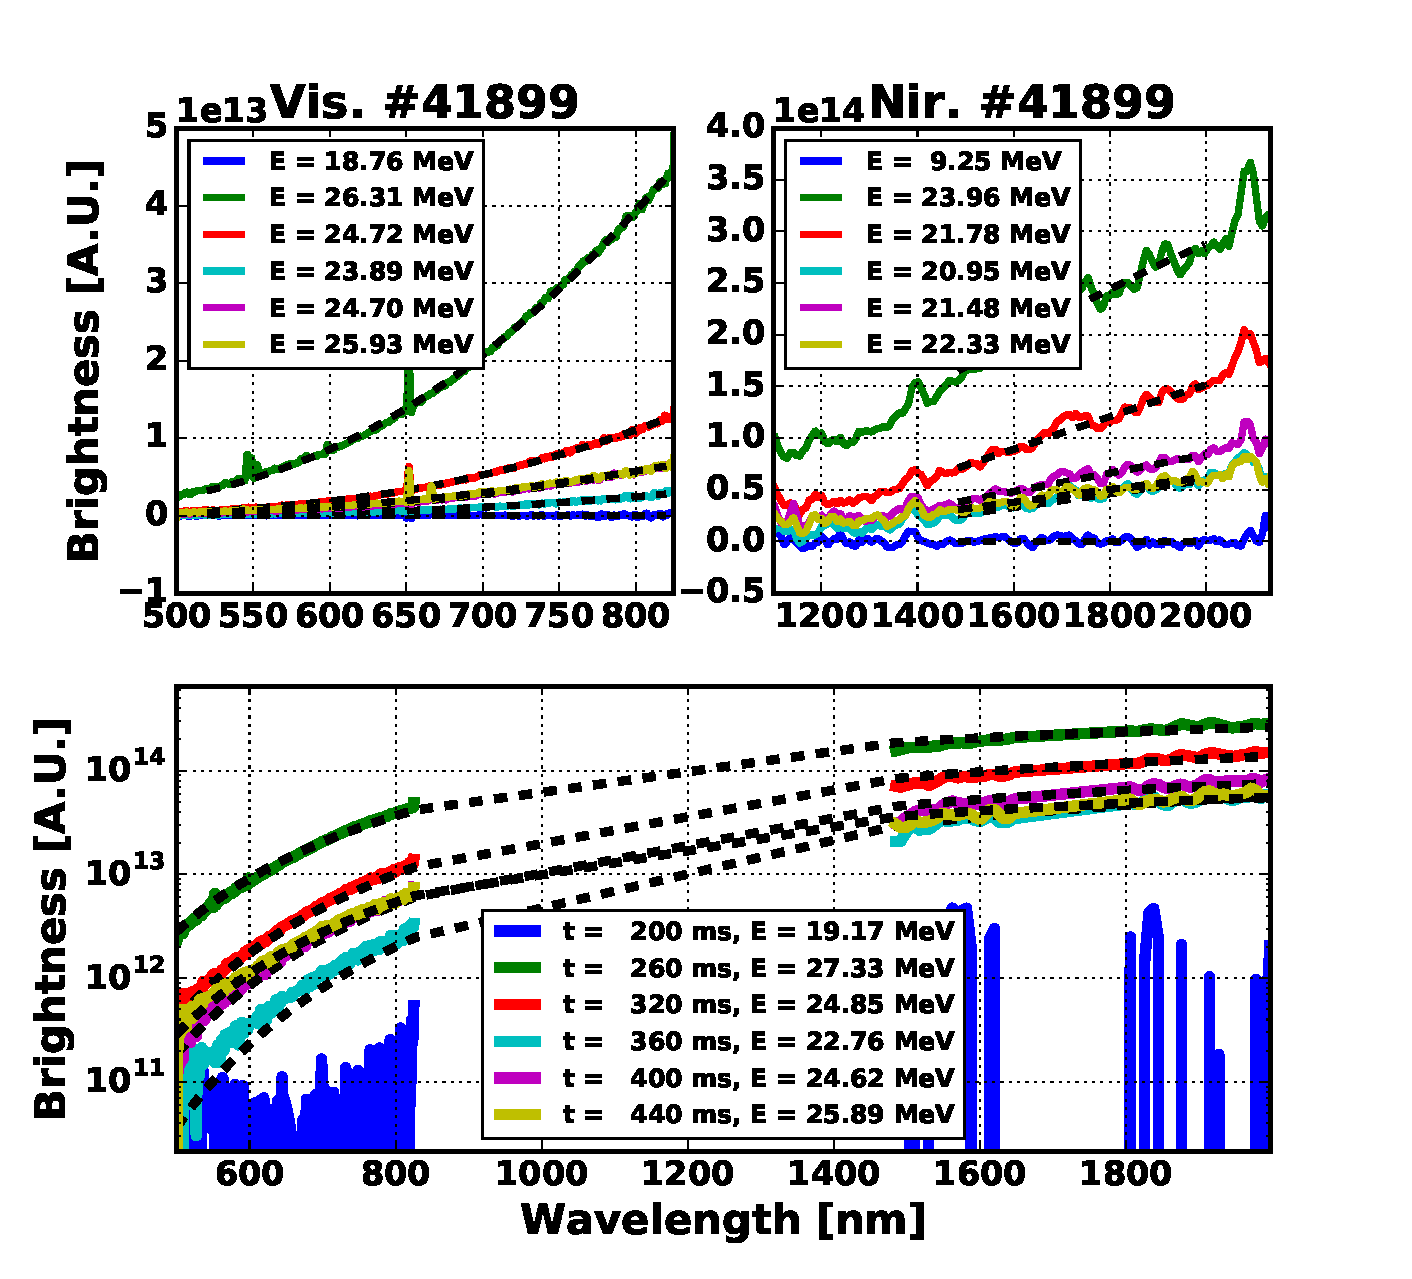
\includegraphics[width=1\textwidth]{chapterreisfig/ftu/41899_fit_.pdf}
        	\end{center}
        \end{figure}
        \scriptsize

        \end{column}
        \end{columns}    
    
    }
    
    \only<2>{
    
        \begin{columns}
        
        \begin{column}{0.5\textwidth}
        
        \scriptsize
        \begin{itemize}
            \item The energy estimation is inferred from: the {\color{green}visible range}, {\color{blue} infrared range} and from the {\color{red} entire spectra}
            \item First pellet at 0.152 s. Second pellet Mo-injection via laser blow-off (LBO) at 0.260 s after the plateau onset.
            \item The energy of the RE beam decrees slowly till 380 ms the energy has a small pick due to the shift toward the HFS of the camera.
            \item The last two pellets (0.479 s and 0.548 s) increase the density of the RE beam and a complete suppression has place as demonstrated by Hard-X signal. 
            \item And finally the beam is lost at about 80 kA. 
        \end{itemize}
        
        \end{column}
        
        \begin{column}{0.5\textwidth}  %%<--- here
        
        \begin{figure}
            \vspace*{-1cm}
        	\begin{center}
                  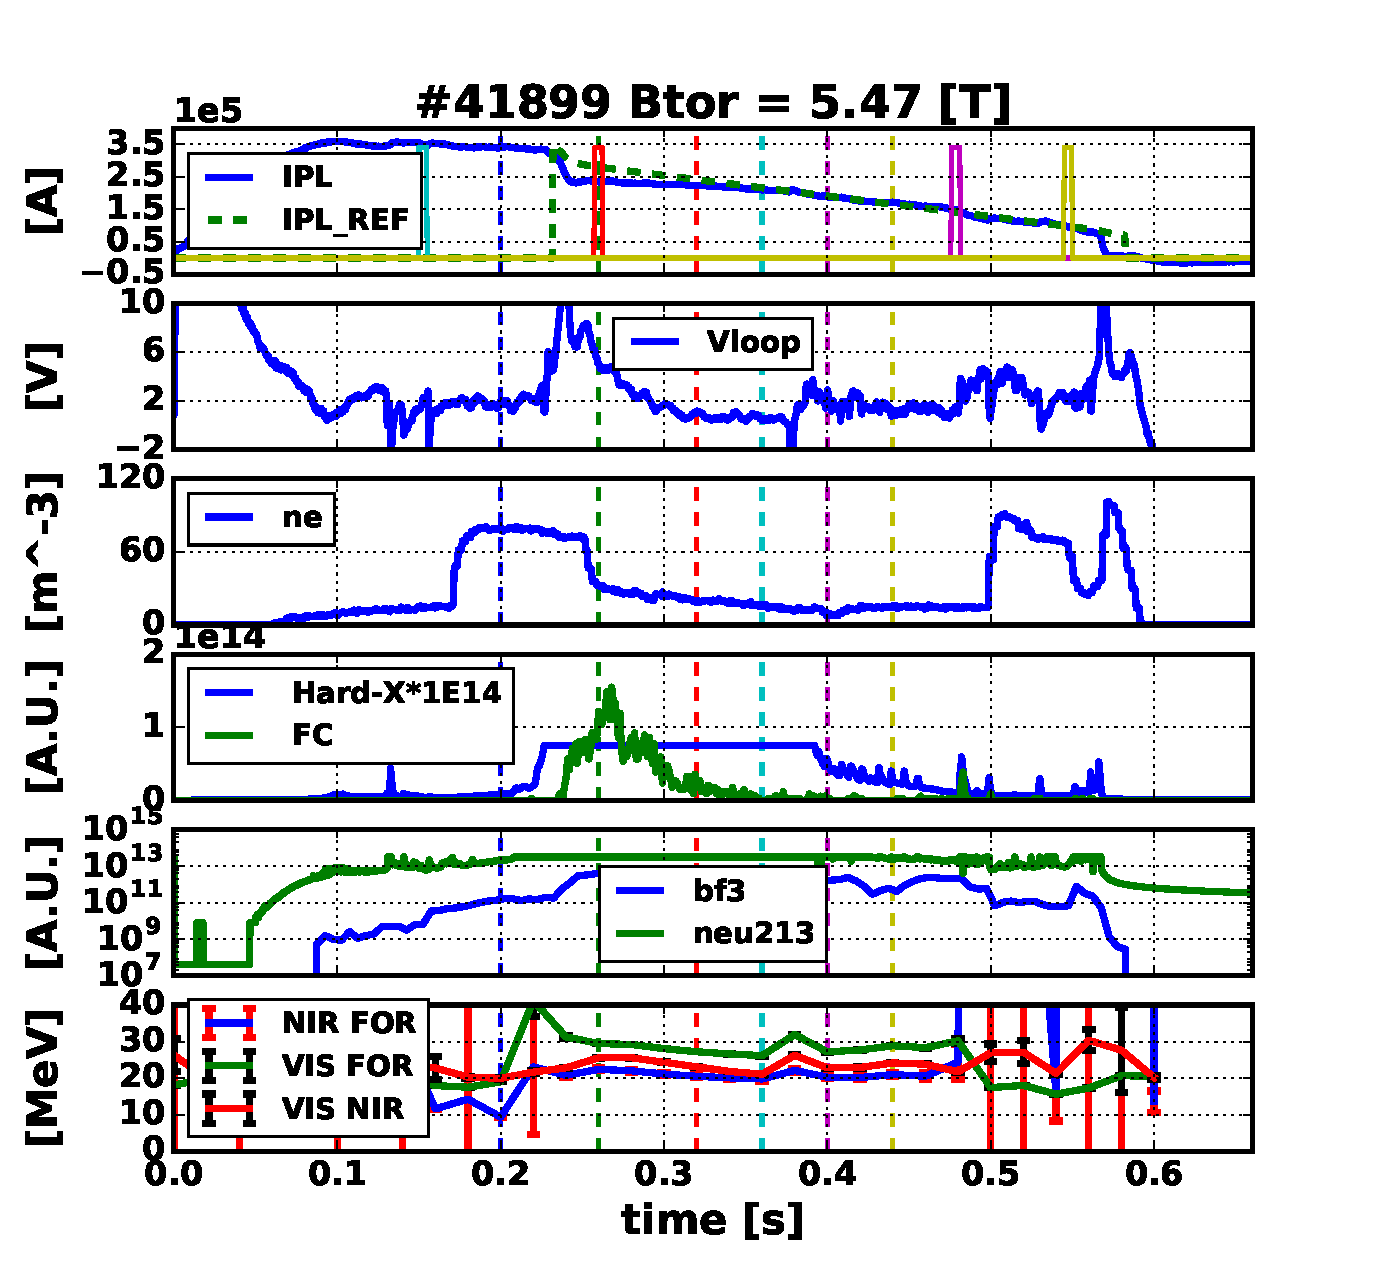
\includegraphics[width=1\textwidth]{chapterreisfig/ftu/41899_ipl_.pdf}
        	\end{center}
        \end{figure}

        \end{column}
        \end{columns}    
    
    }
    
    
\end{frame}





\begin{frame}{AUG: Experimental results}

\only<1>{
    \begin{columns}
    	\begin{column}{0.5\textwidth}
    	     \begin{center}
    	
    				\begin{figure}
    					\vspace*{-1cm}
    					\begin{center}
    						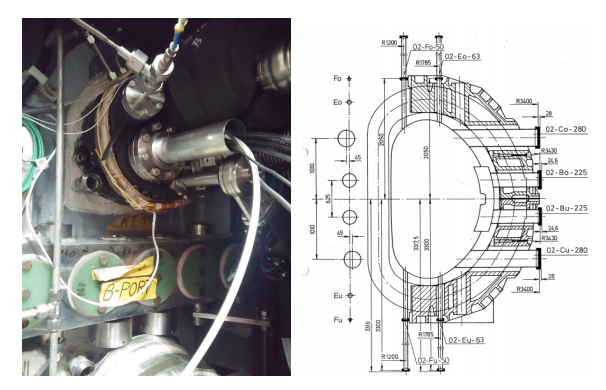
\includegraphics[width=0.8\textwidth]{chapterreisfig/aug_port.png}\\
    						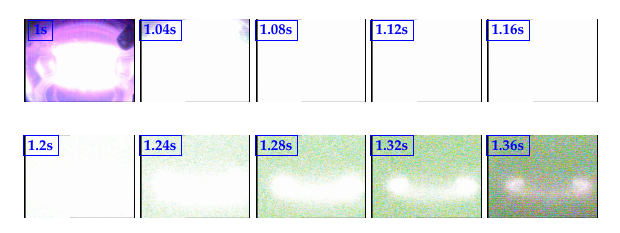
\includegraphics[width=1\textwidth]{chapterreisfig/asdex/image_34183_.png}
    					\end{center}
    				\end{figure}
    
    	
    	     \end{center}
    	\end{column}
    	\begin{column}{0.5\textwidth}  %%<--- here
    	
    	\begin{figure}
    		\vspace*{-1cm}
    		\begin{center}
                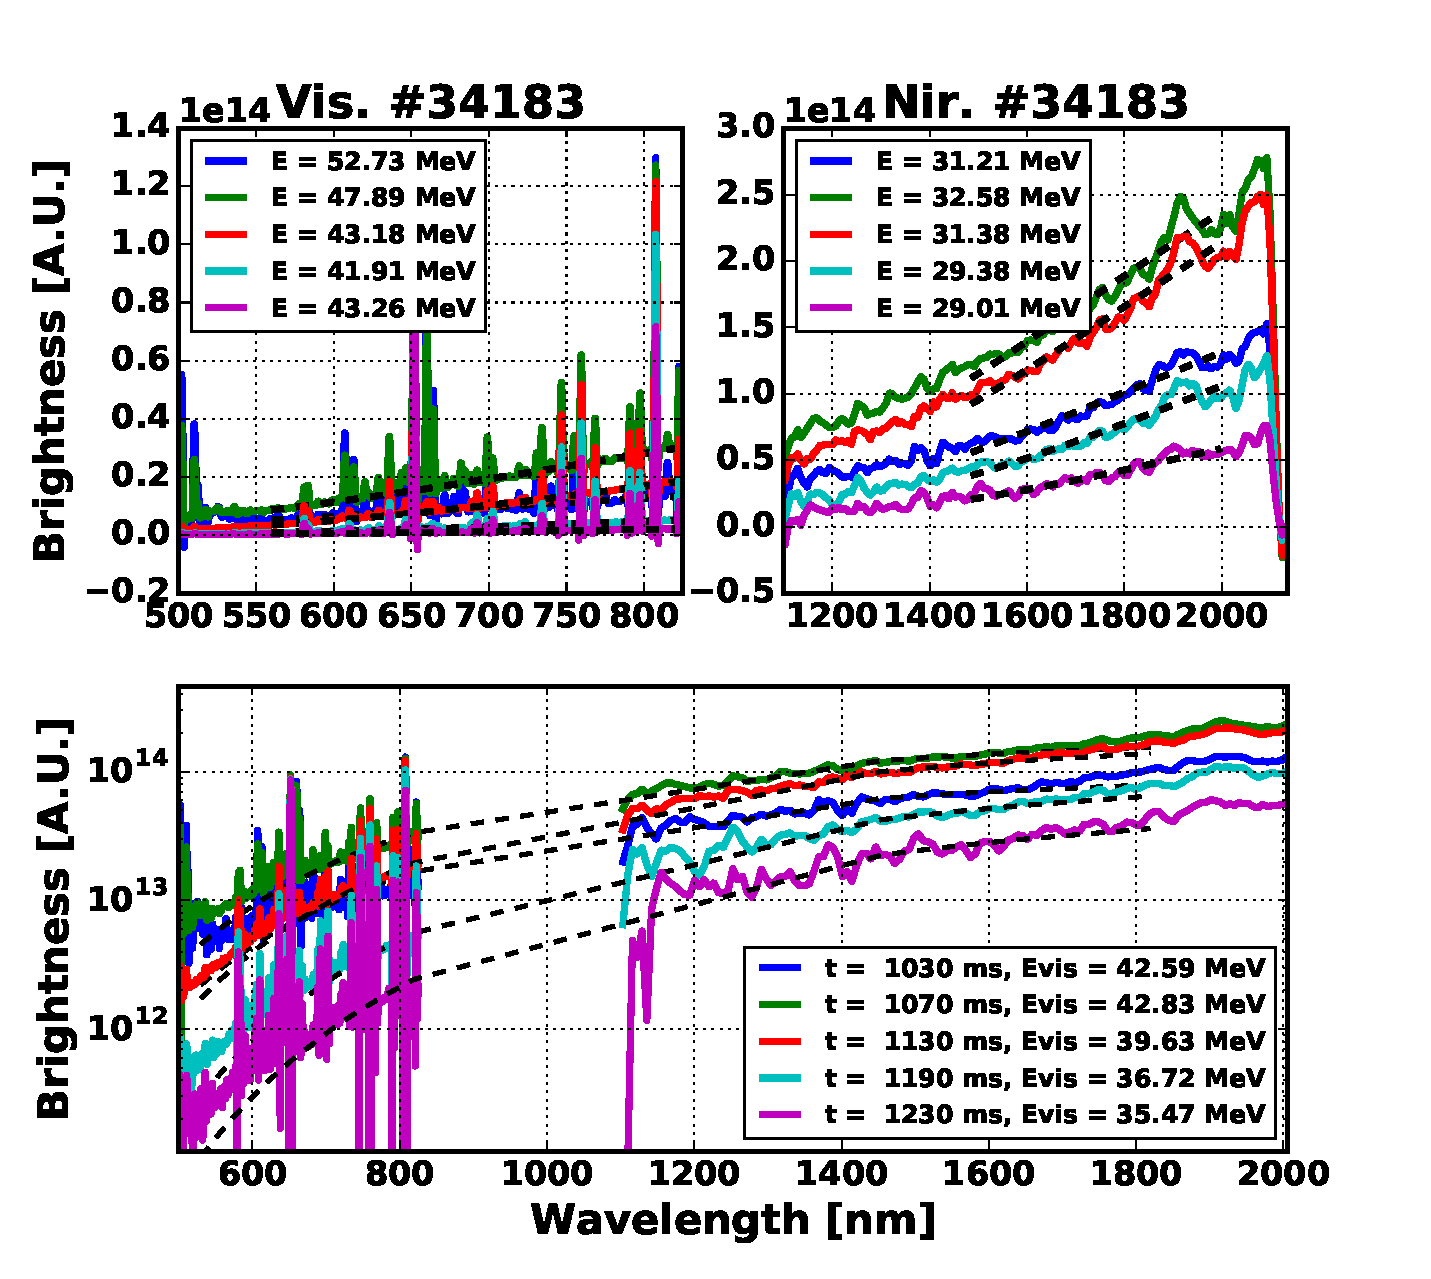
\includegraphics[width=1\textwidth]{chapterreisfig/asdex/34183_fit_.pdf}
            \end{center}
    	\end{figure}
    	
    	\end{column}
    \end{columns}
}

\only<2>{
    \scriptsize
    \begin{itemize}
        \item     Discharge \#34183 performed at 2.48 \si{\tesla}.\\
        \item     Deuterium pellets(1.9x1.9x2.0 \si{\mm}; $n_e$ = 4.3e20) were injected from 1.02 \si{\s} at 70 \si{\Hz}\\
        \item     After 1250 \si{\ms} the data are subjected to a high variance.

    \end{itemize}

	\begin{figure}
		\vspace*{-.1cm}
		\begin{center}
            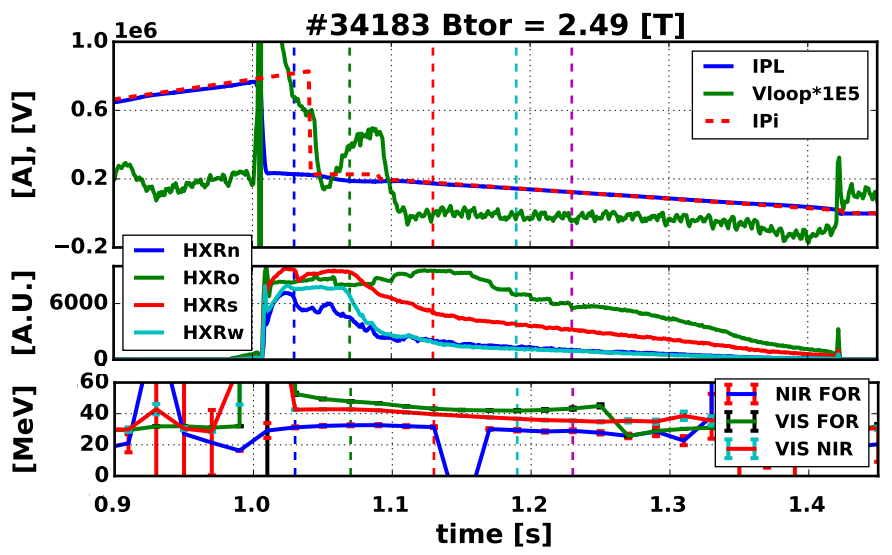
\includegraphics[width=0.8\textwidth]{chapterreisfig/asdex/asdex_34183.png}
        \end{center}
	\end{figure}

}

\end{frame}


\begin{frame}{TCV: Experimental results}
    \begin{columns}
    	\begin{column}{0.4\textwidth}
    	     \scriptsize
    	     \begin{left}

        	     \begin{itemize}
        	        \only<1>{
        	        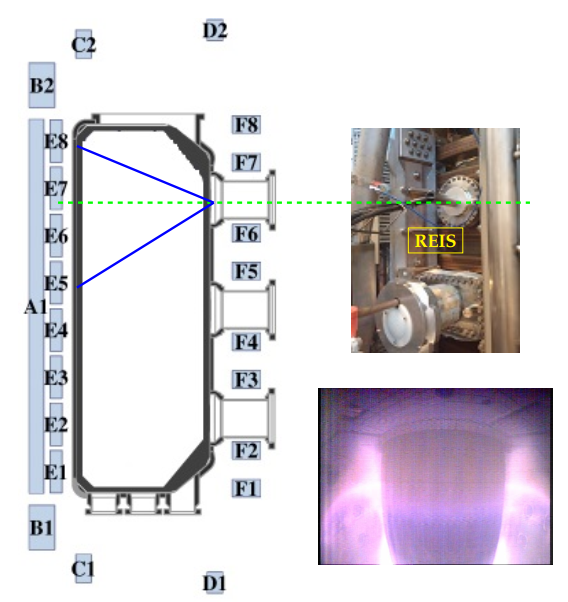
\includegraphics[width=0.8\textwidth]{chapterreisfig/tcv_port.png}
        	        }
        	        \only<2>{
        	            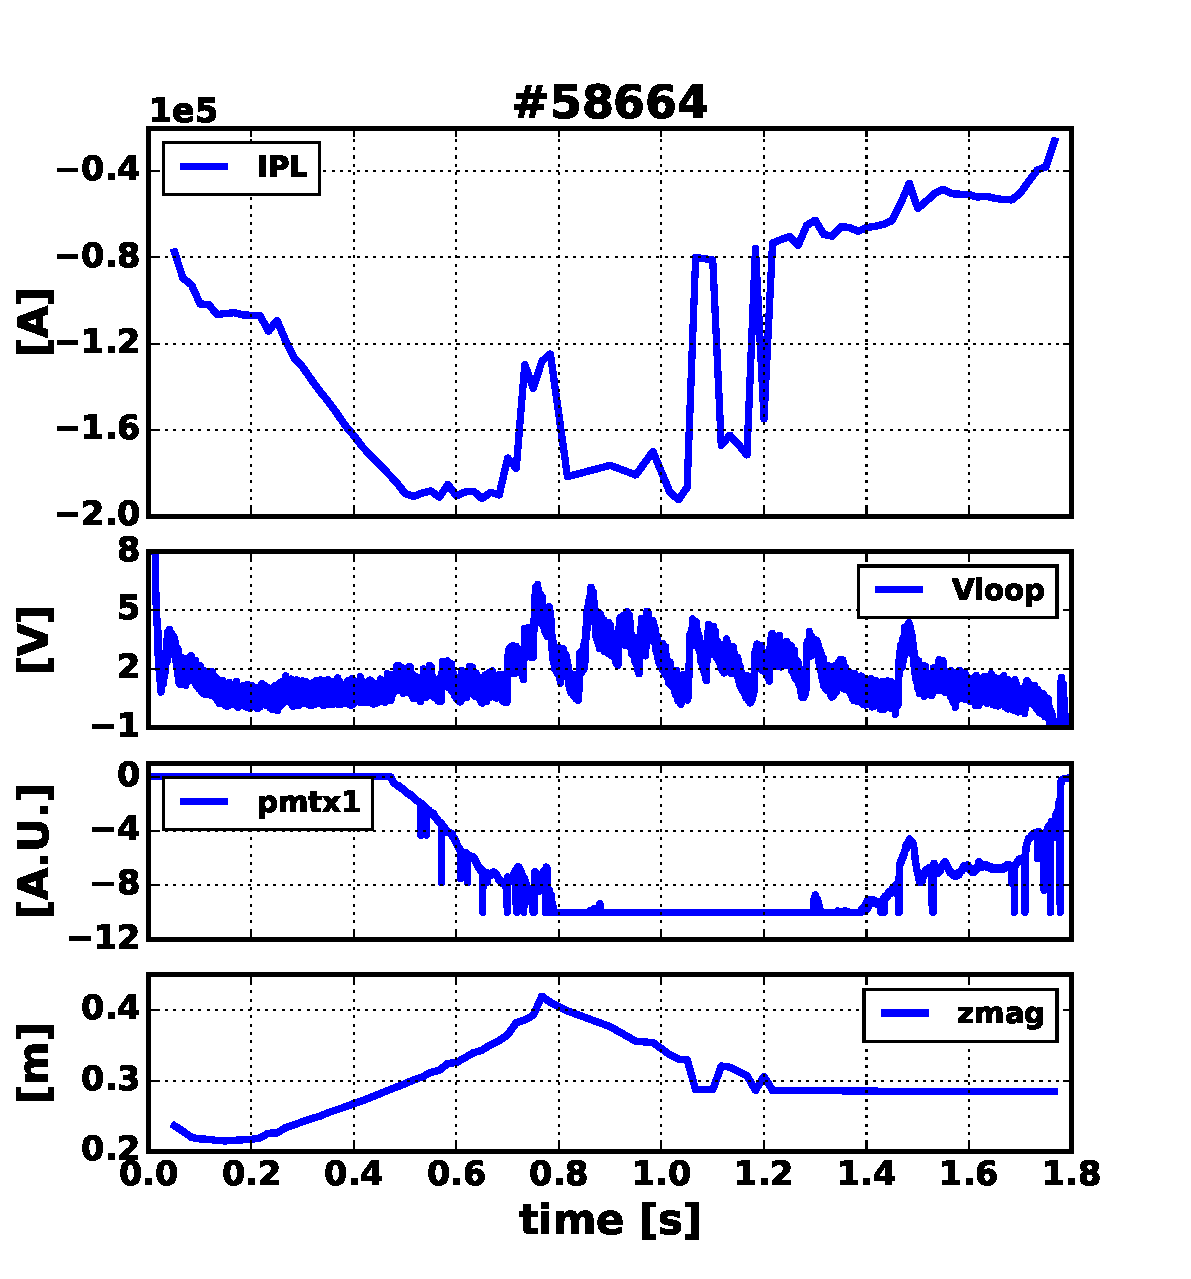
\includegraphics[width=0.9\textwidth]{chapterreisfig/tcv/ipl_58664_.pdf}
        	        }
        	     \end{itemize}

    	     \end{left}
    	\end{column}
    	\begin{column}{0.6\textwidth}  %%<--- here
    	
    			\begin{figure}
    				\begin{center}
    					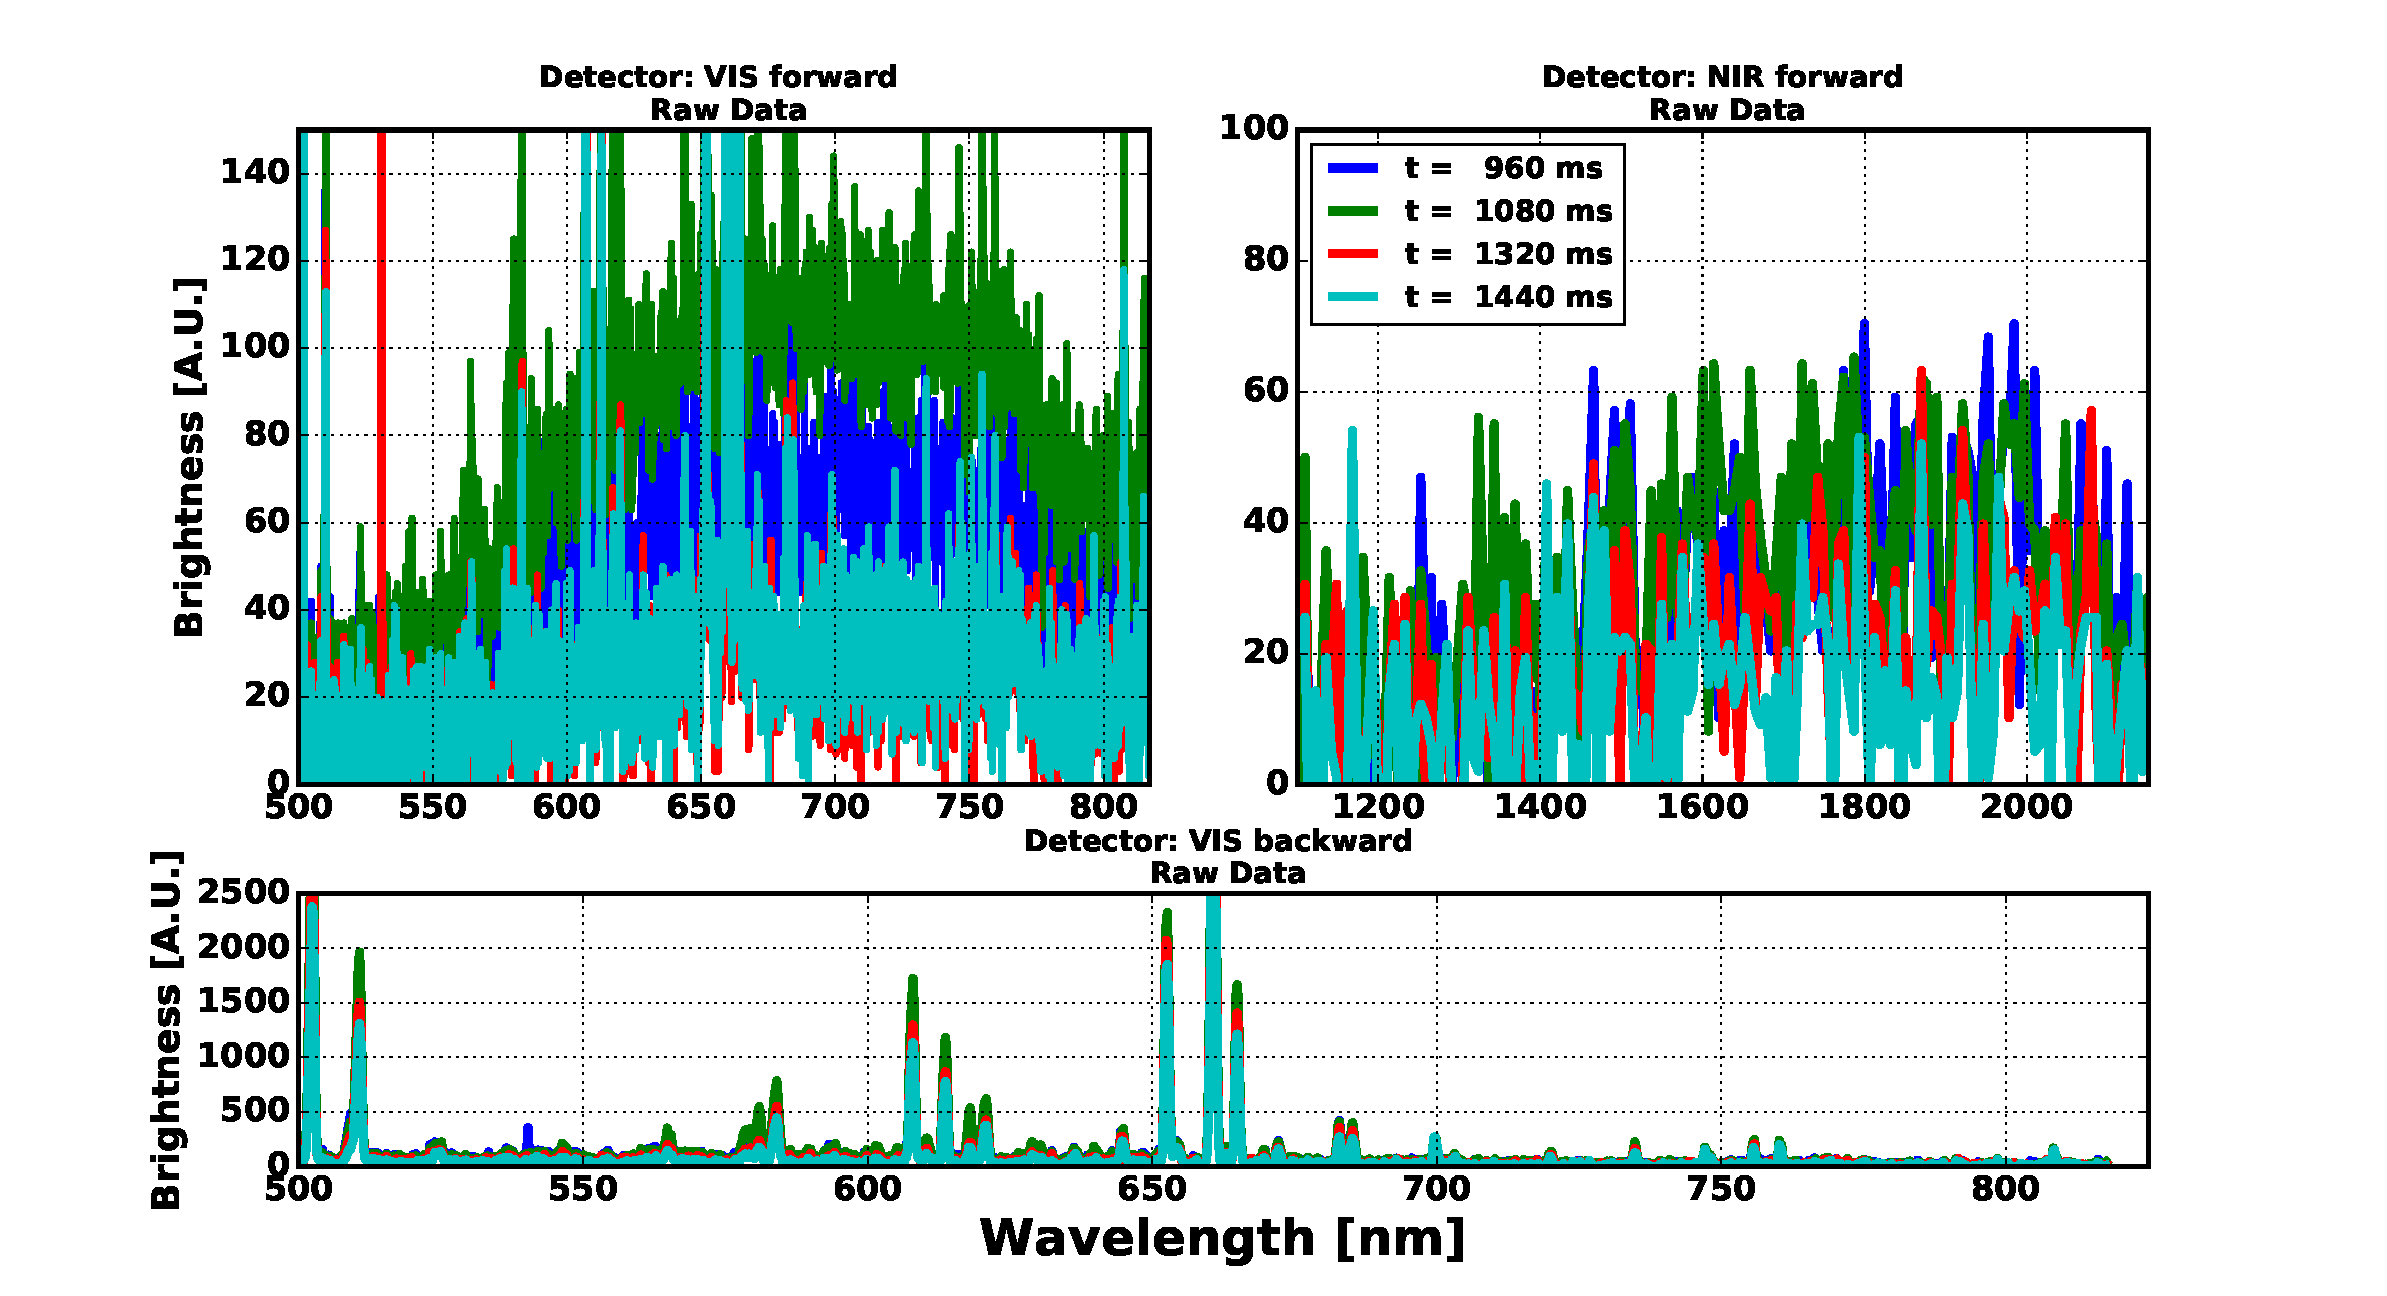
\includegraphics[width=0.9\textwidth]{chapterreisfig/tcv/spectra_58664_.pdf}
    				\end{center}
    			\end{figure}
    	
    	\end{column}
    \end{columns} 

\end{frame}


%------------------------------------------------------------------------------

\section{Real-time elaboration system for two-color scanning interferometer}
\begin{frame}{Interferometer: introduction}
\scriptsize	
\begin{itemize}
\item Developing of a new \textbf{real-time acquisition and elaboration system} that calculates the line averaged density using the two-color scanning beam interferometer(\cite{doi:10.13182/FST04-A522}).
\item \textbf{The main goal} of the real-time acquisition system is the estimation of the radial displacement of the RE beam during the plateau phase.
\end{itemize}

\begin{columns}
	\begin{column}{0.5\textwidth}
                \centering
                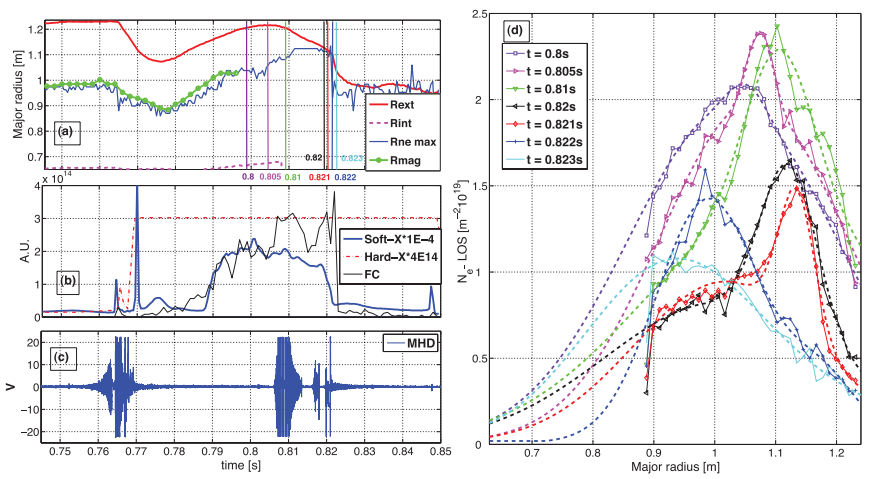
\includegraphics[width=1\linewidth]{inter/density_profile_35965_}	\end{column}
	\begin{column}{0.5\textwidth}  %%<--- here
	
        \begin{figure}
        	\centering
        	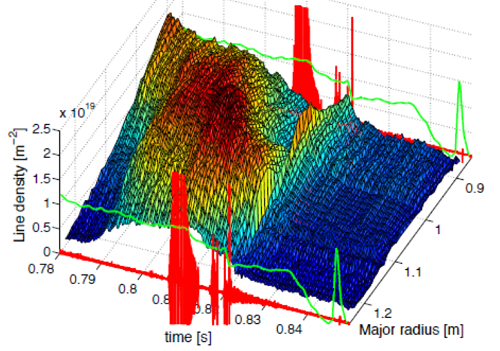
\includegraphics[width=0.8\textwidth]{inter/inter_35965.png}
        \end{figure}
    \scriptsize	

	\end{column}
\end{columns} 	

\begin{itemize}
    \item RE beam is enveloped by cold electrons (\textbf{assumption}) and that the interferometer is able to estimate the radial displacement.
    \item The radial profiles of the line integrals can be fitted with Gaussian functions (least square minimization)
\end{itemize}

		
\end{frame}	


\begin{frame}{Interferometer: Two colour scan interferometer}
\scriptsize
Layout of a two-color scanning interferometer: poloidal section of the path of the scan beam.
$$n_e(t) = \frac{3.55\times10^{14}}{L} \frac{\lambda_1 \Phi_1(t)-\lambda_2 \Phi_2(t)}{\lambda^2_1-\lambda^2_2}$$  where $L$ is the length of the LOS, $\phi_1(t)$ and $\phi_2(t)$ are the phase shifts at time $t$, $\lambda_1$= 10.6$\mu m$ is the main wavelength (CO2) and $\lambda_2$=5.4$\mu m$ (CO).
\begin{figure}
    %\vspace*{-1cm}
	\centering
	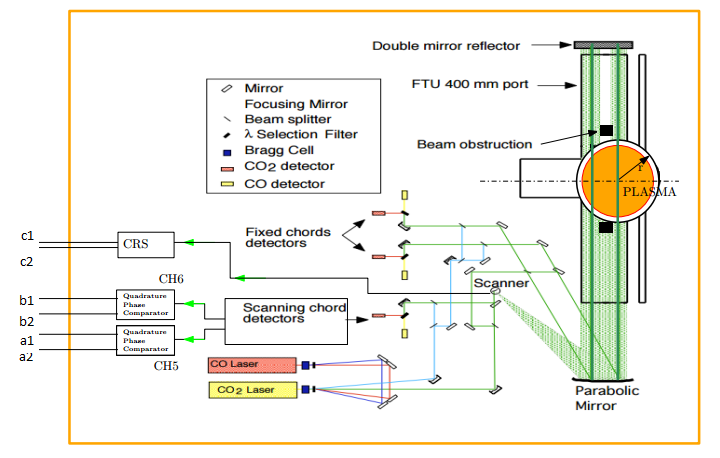
\includegraphics[width=0.7\textwidth]{inter/interf_HARDWARE.png}
\end{figure}


\end{frame}


\begin{frame}{Interferometer: Real-time architecture}
\scriptsize
The acquisition system is based on \textbf{MARTe} framework (Multi-threaded Application Real-Time executor)

\begin{columns}
	\begin{column}{0.4\textwidth}
	    \begin{center}
	    
        \begin{itemize}
        	\item {\color{red} The IOGAMs:\\
        	+AD20xxTimeInputGAM, +RFMInputGAM and +SynchOutputGAM.}
        	\item  {\color{blue} The GAMs:\\
        	+CollectionGAM and +DensityGAMCHX.}
        	\item Three high speed acquisition boards (10 channels at 1.5 $MHz$) externally synchronized by mean of 30 MHz clock and gate signal.
        	\item Density elaboration of 32 SOL every 1.5ms.
        \end{itemize}    
	    
    	\end{center}
    	\end{column}
    	\begin{column}{0.6\textwidth}
            \begin{figure}
                \vspace*{-0.8cm}
            	\centering
            	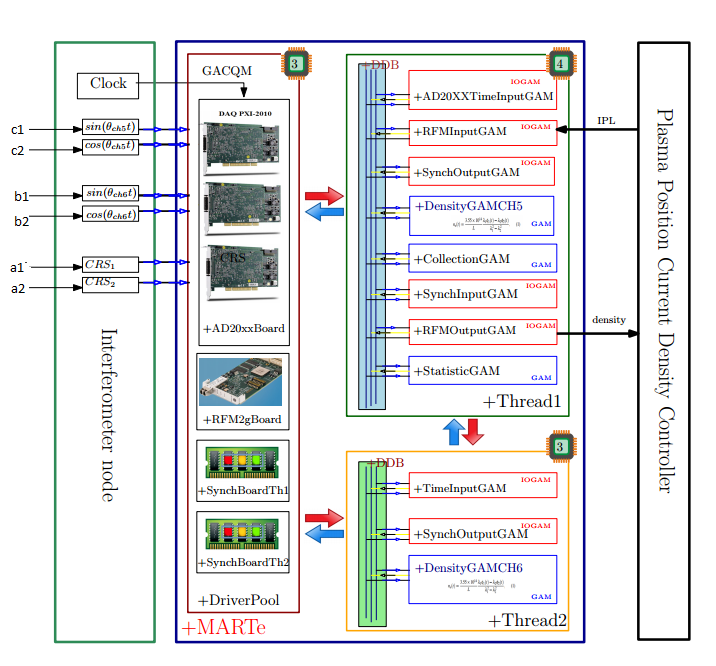
\includegraphics[width=1\textwidth]{inter/interf_MARTe.png}
            \end{figure}
        \scriptsize	
    \end{column}
\end{columns} 


\end{frame}


\begin{frame}{Real-time interferometer: Experimental results}
    \begin{figure}
        \centering
        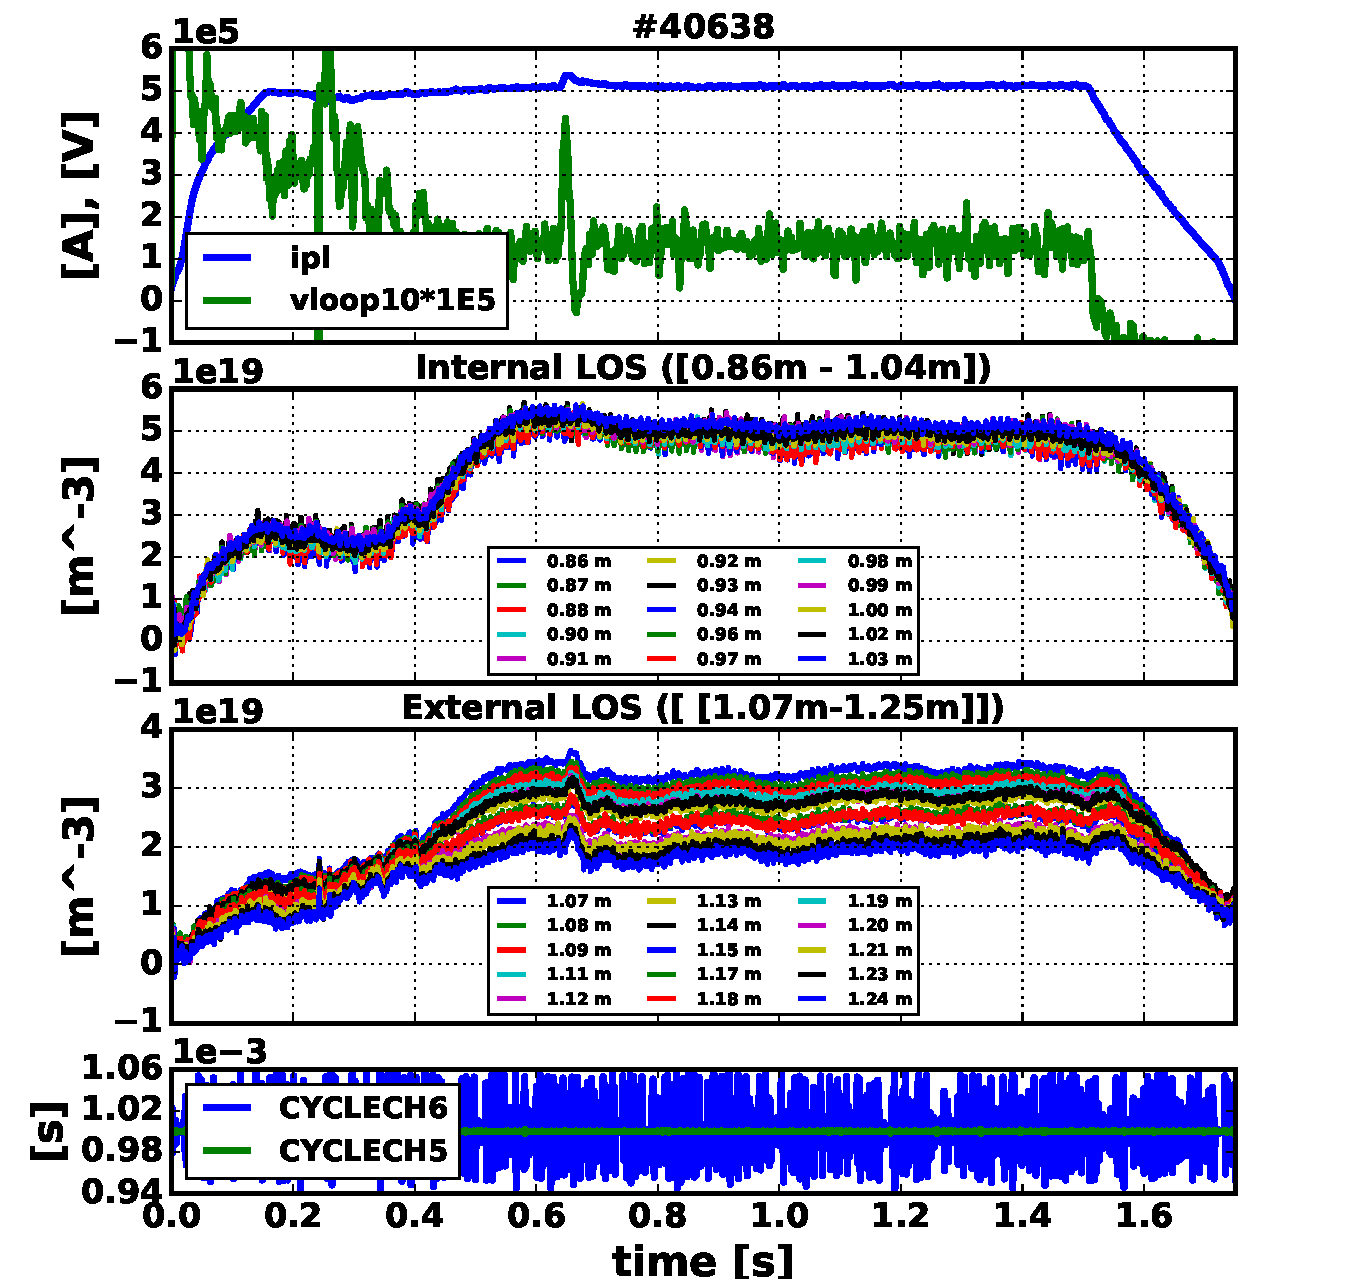
\includegraphics[width=0.7\textwidth]{inter/inter_40638.pdf}
    \end{figure}
    
    
\end{frame}





%------------------------------------------------------------------------------
\section{Runaway electrons control system (RECS)}

\begin{frame}{RECS: Introduction}

\begin{figure}[h]
	\centering
	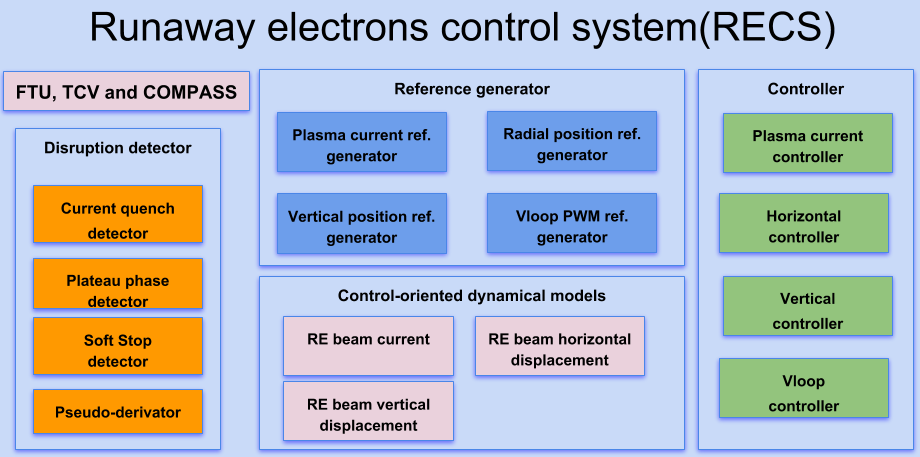
\includegraphics[width=1\linewidth]{Chapter3Fig/RESCframework.png}
\end{figure}
\end{frame}


\begin{frame}[allowframebreaks]{RECS: Control oriented models of plasma current}
\scriptsize
\begin{equation}
	\dot{I}_p = -p_1I_p - p_2\dot{I}_V -p_3 \dot{I}_T - p_4FC,
\end{equation}
The parameter $p_1 = \frac{R}{L}$ approximates the exponential decay rate of the plasma current, $I_V$ and $I_T$ are respectively the current flowing in the coils V and T coupled with the RE current via the mutual inductance $p_2$ and $p_3$ between the plasma and the coils. And $FC$ is a measurement related to the RE lost on the vessel.\\

\begin{columns}
	\begin{column}{0.6\textwidth}
        \begin{figure}
        \vspace*{-0.8cm}
        \centering
            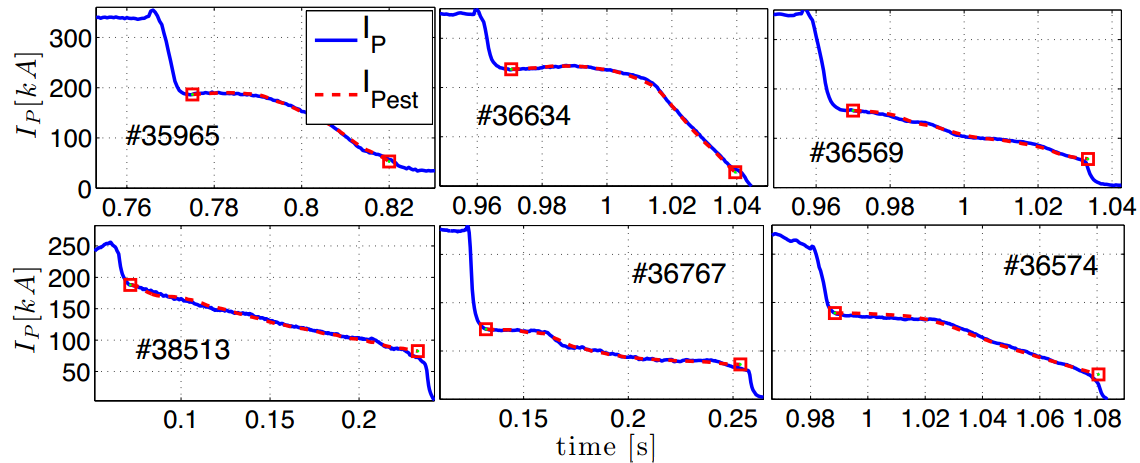
\includegraphics[width=1\textwidth]{models/ipl.png}
        \end{figure}
    \end{column}
    \begin{column}{0.4\textwidth}
\begin{table}
	\tiny
	\begin{center}
		\begin{tabular}{ | l | l | l | l |}
			\hline
			params & $\overline{x}$ & $\sigma$ & SI base unit\\ \hline
			$p_1$ & 6.7 & 1.6 & \si{\s} \\ \hline 
			$p_2$ & 7.5 & 8.9 & - \\ \hline
			$p_3$ & 2.7 & 1.8 & - \\ \hline 
			$p_4$ & 1.3E-9 & 1.3E-9& $\frac{A}{s}$ \\ \hline 
		\end{tabular}
	\end{center}
\end{table}	
    \end{column}
    
\end{columns}

\end{frame}


\begin{frame}{RECS: Control oriented models of radial displacement}
    
    
    \scriptsize
    
    \begin{equation}
    \left\{
    \begin{array}{ll}
    \dot x_1= x_2,\\
    \dot x_2= \!{-}c_1x_1\!{-}c_2x_2\!{+}((c_3(3.8I_V\!{+}I_F)\!{-}c_4I_p)\!{+}c_0)\!{+}c_5x_3, 	\\
    \dot x_3 =\!\!{-}c_6x_3\!{+}(V_{\text{loop}}\!{-}c_7),
    \end{array}
    \right.
    \end{equation}
    
where $x_1$ is the estimated $R_{\text{ext}}$ and $x_2$ its time derivative.
The balance term $((c_3(3.8I_V+I_F)-c_4I_p)+c_0)$ is close to zero in equilibrium conditions accounting for the vertical magnetic fields produced by the current in the coil F, V, and the one generated by $I_p$ (\cite{Astolfi2014}). The term $c_5x_3$ introduces the radial-shift since
$x_3$ is a rough estimate of the RE energy that is a function of the loop voltage $V_{loop}$, collisional damping as well as the synchrotron radiation losses that are roughly accounted by the constant term $c_7$ (\cite{Martin-Solis2010}).
    
\begin{columns}

	\begin{column}{0.6\textwidth}
        \begin{figure}
        \vspace*{-0.8cm}
        \centering
        	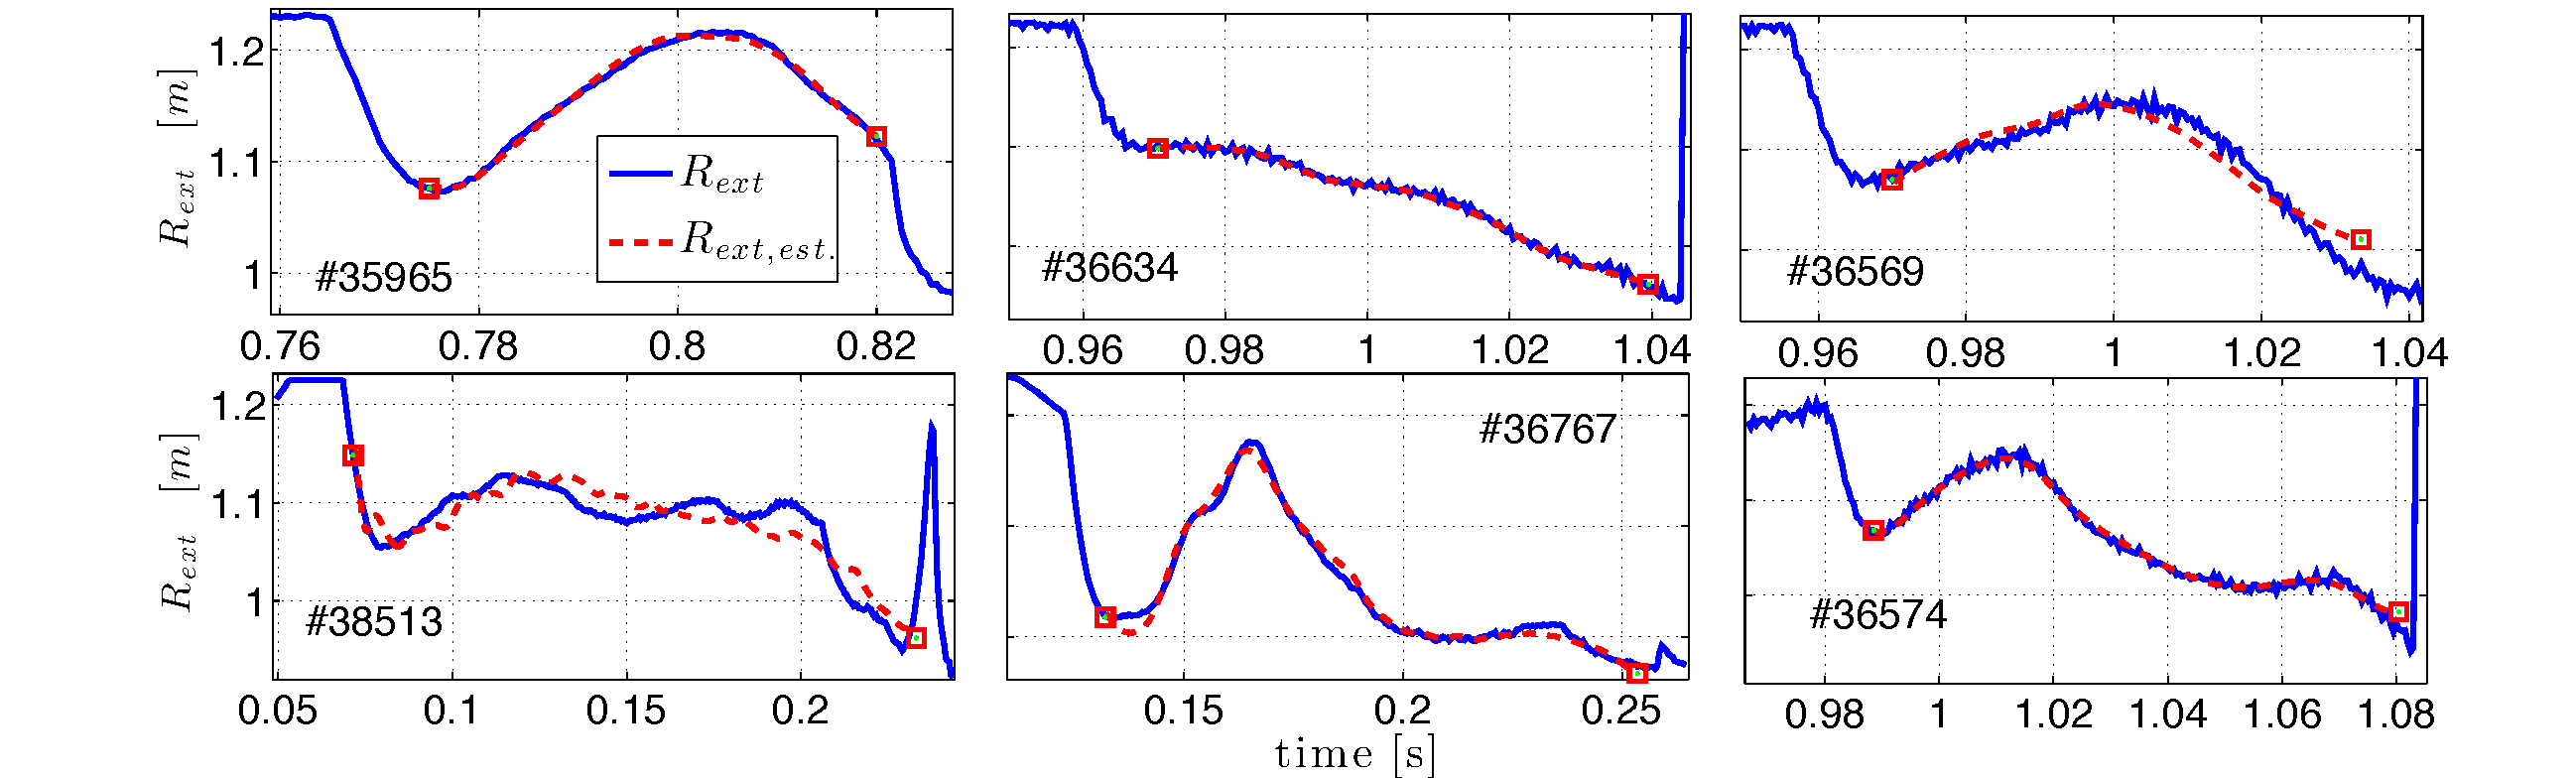
\includegraphics[width=1\textwidth]{models/rs2}
        \end{figure}
    \end{column}
    
    \begin{column}{0.4\textwidth}
\begin{table}
	\tiny
	
	\begin{center}
		\begin{tabular}{| l | l | l | l |}
			\hline
			params & $\overline{x}$ & $\sigma$ & SI unit base \\ \hline
			$c_0$ & 0.0 & 0.0 & $\frac{m}{s^2}$ \\ \hline
			$c_1$ & 4.3E3 & 1.8E3 & $\frac{1}{s^2}$ \\ \hline
			$c_2$ & -2.9E6 & 8.6E5 & $\frac{1}{s}$ \\ \hline
			$c_3$ & -0.81 & 1.2 	& $\frac{m}{s^2A}$ \\ \hline
			$c_4$ & 23 & 21 & $\frac{m}{s^2A}$ \\ \hline
			$c_5$ & 6.7E5 & 1.6E5 & $\frac{m}{s^2V}$ \\ \hline
			$c_6$ & 6.6E-3 & 0.3 & $\frac{1}{s}$ \\ \hline
			$c_7$ & 1 & 0.0 & $\frac{J}{sV}$ \\ \hline
			$c_8$ & 3.6 & 2.0 & $\frac{J}{s}$ \\ \hline
		\end{tabular}
	\end{center}
\end{table}
    \end{column}
    
\end{columns}

\end{frame}



\begin{frame}{RECS: RE beam control strategy}
	\tiny
		The main strategy, when a RE beam is detected, consists in ramping down the RE beam current to dissipate its energy through the central solenoid.
		\begin{itemize}
    		\item The new plasma current references is computed as:
            \begin{equation}
             I^{Ref} += \gamma I^{Ref} + (1-\gamma) I_{linear}^{Ref};
            \end{equation}
            where $\gamma$ is the eigenvalue of the discrete first order system while $I_{linear}^{Ref}$ is the linear reference computed during the plateau phase as 
            \begin{equation}
            I_{linear}^{Ref} = I_P(t_{plateau}) - \alpha (t-t_{plateau}); 
            \end{equation}
    		
    		
    		\item reduce the external reference ($R_{ext}$) during the CQ phase and also during the ramp-down safety shot-down policy when the XHR signal exceed a specific threshold for a given time (10 ms in FTU).
    		The new references is computed as:
            \begin{equation}
             R_{ext}^{Rif} = \gamma R_{ext}^{Rif} + (1-\gamma) R_{ext}^{IP};
            \end{equation}
            where $R_{ext}^{Rif} \in [R_{ext}^{MIN},R_{ext}^{MAX}]$ is limited between $R_{ext}^{MIN}$ and $R_{ext}^{MAX}$ for security reasons, $\gamma$ is the time constant of the first order and $R_{ext}^{IP}$ is computed as 
            \begin{equation}
             \label{eq:Rextneq}
             R_{ext}^{IP} = R_{offset}^{Rif} + T_{min} + \gamma + \frac{I_P}{I_P(t_{plateau})} (R_{ext}(t_{plateau})- T_{min})
            \end{equation}
		\end{itemize}

\end{frame}

\begin{frame}{RECS: FTU Post-disruption RE beam suppression}

    \begin{figure}[h]
    	\vspace*{-2cm}
        \centering
        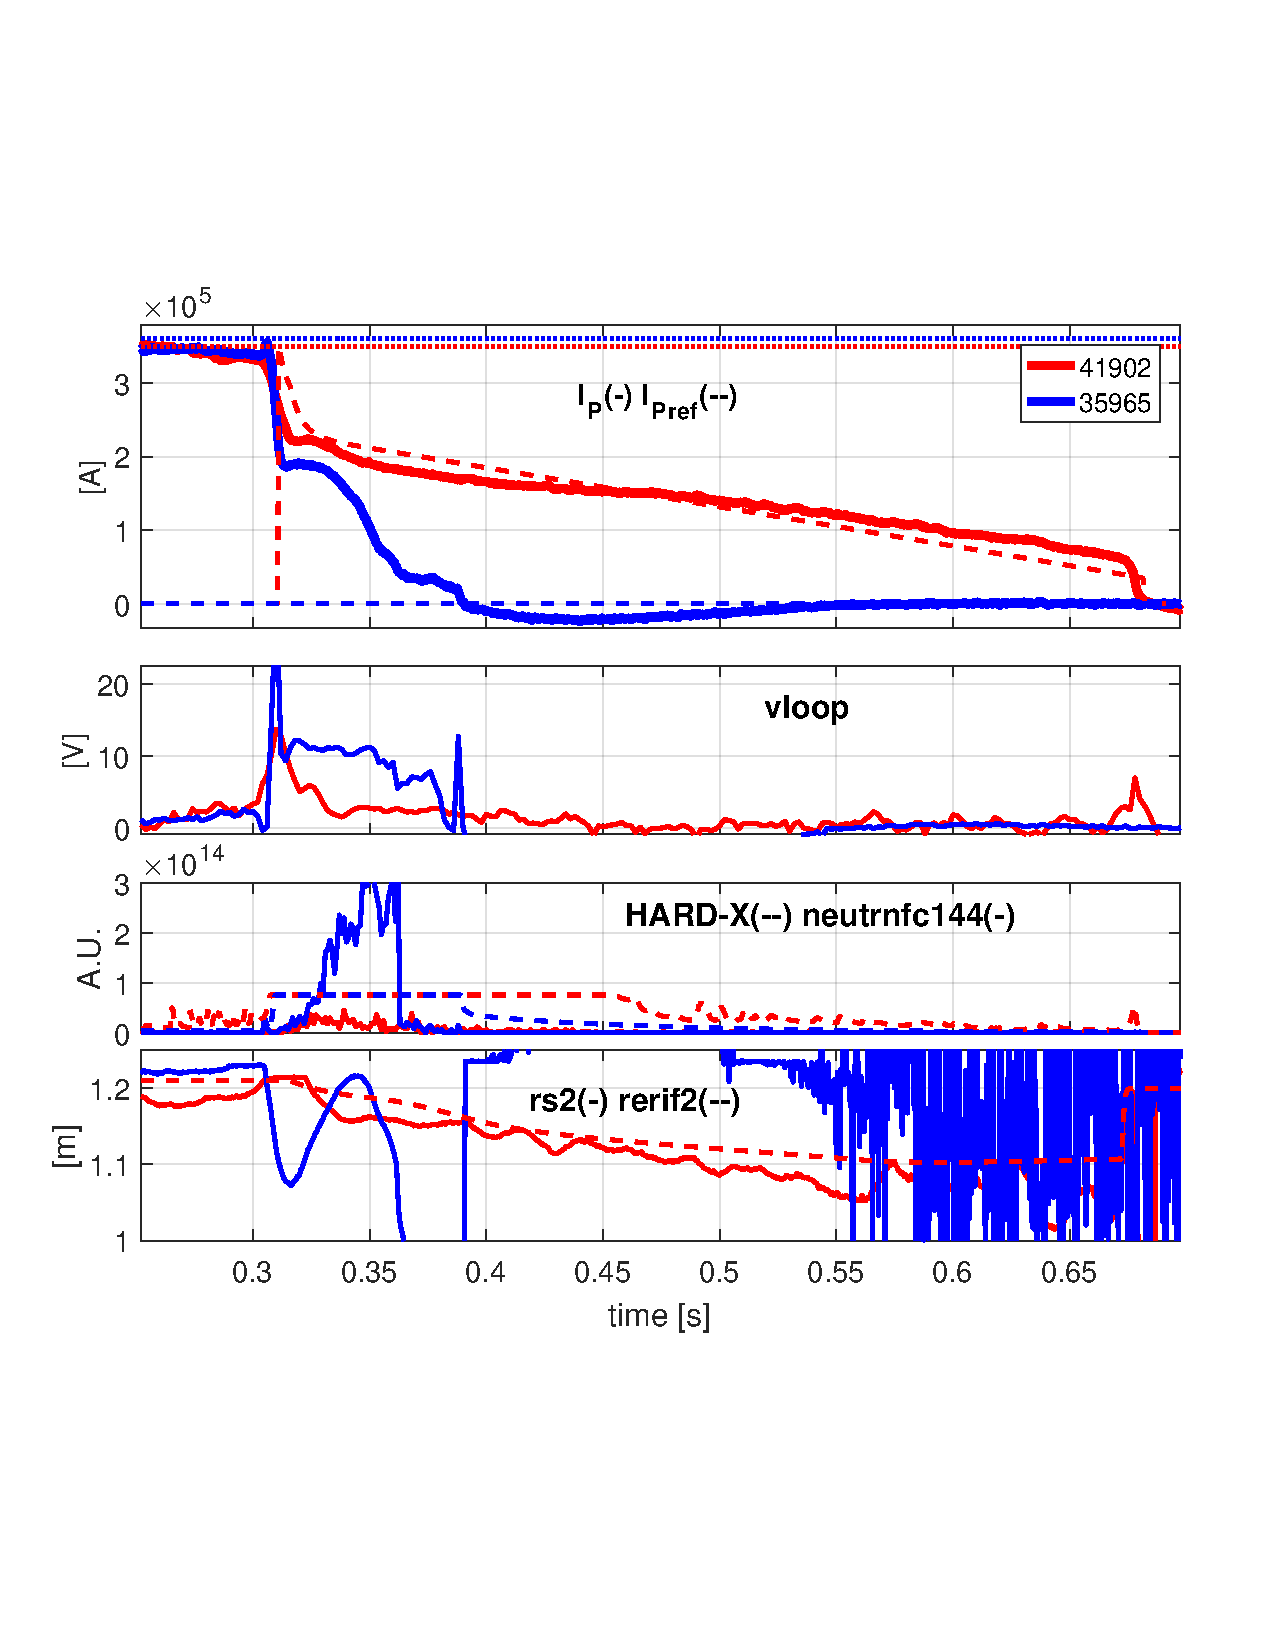
\includegraphics[width=0.7\linewidth]{Chapter3Fig/example.pdf}
    \end{figure}

\end{frame}


\begin{frame}{RECS: TCV Post-disruption RE beam suppression}
    \centering
    \only<1>{
    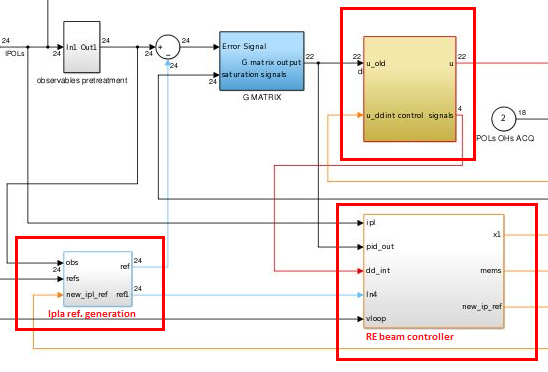
\includegraphics[width=0.8\linewidth]{fig/tcv_scheme_zoom.png}
    }
    \only<2>{
    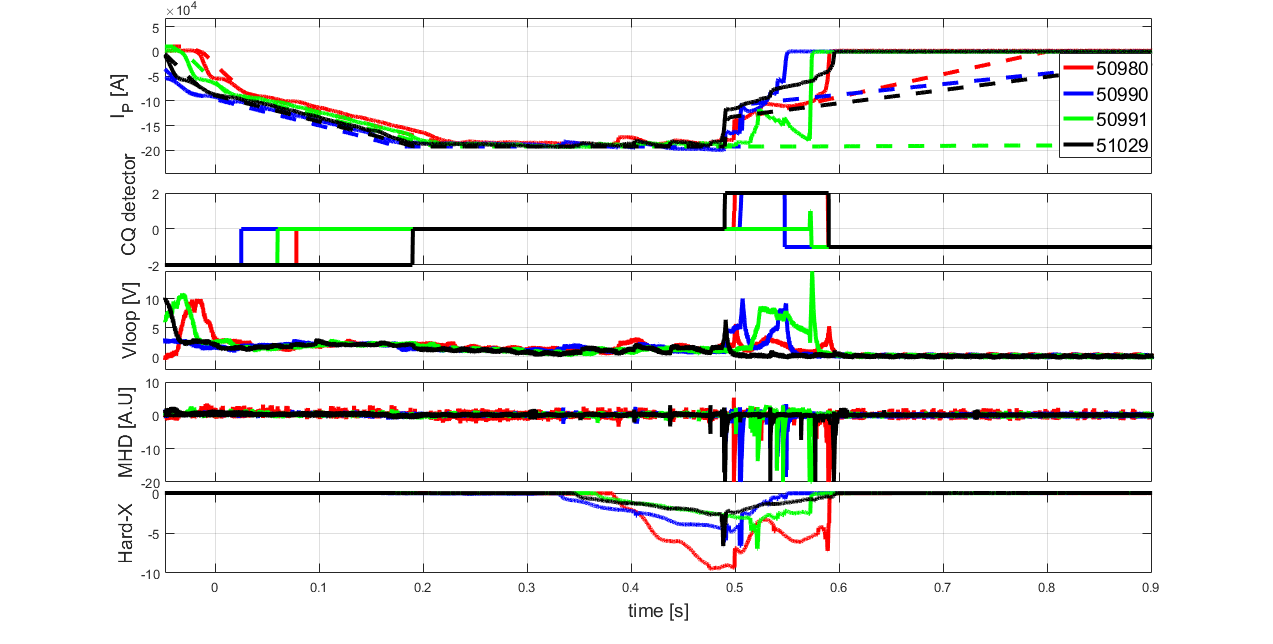
\includegraphics[width=1\linewidth]{fig/50980to51029_1.png}
    }
    \only<3>{
    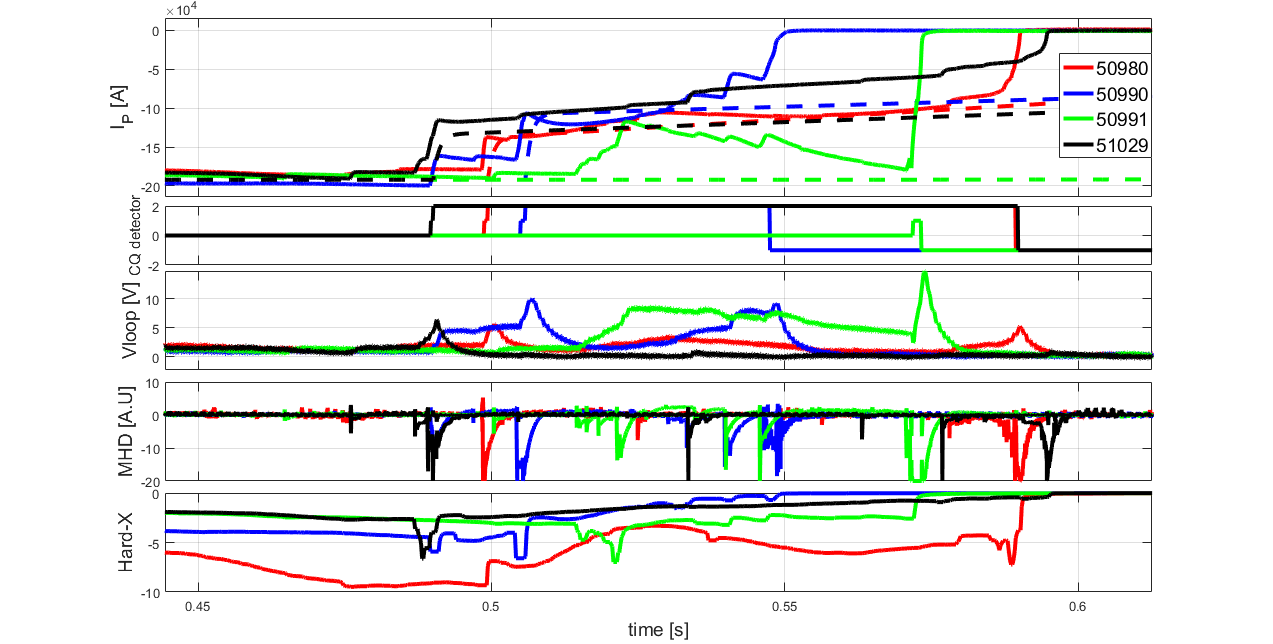
\includegraphics[width=1\linewidth]{fig/50980to51029_2.png}
    }
\end{frame}



%------------------------------------------------------------------------------
\section{Summary}
\begin{frame}{Summary}
    \scriptsize
	\begin{itemize}
		\item REs data analysis: hysteresis phenomena.
    	\item REIS SYSTEM: data analysis, installation (FTU, AUG and TCV), calibration, data acquisition development and energy estimation.
		\item Development of a real-time acquisition system of a two-color scanning beam interferometer.
		\item (RECS) framework: Control-oriented models, Post-disruption RE beam suppression (FTU, COMPASS and TCV), FTU Vloop oscillations, FTU plasma elongation control.
	\end{itemize}
\end{frame}

\begin{frame}[allowframebreaks]
\frametitle{References}
\tiny
\bibliographystyle{abbrvnat}
\bibliography{ref}
\end{frame}





\end{document}


